\documentclass[final,3p,times,number]{elsarticle}
\usepackage[utf8]{inputenc}
\usepackage{graphicx}
\usepackage{booktabs}
\usepackage{array}
\usepackage{tabularx}
\usepackage{multirow}
\usepackage{amsmath}
\usepackage{amssymb}
\usepackage{placeins}
\usepackage{float}
\usepackage[font=small,skip=6pt]{caption}
\usepackage{subcaption}
\usepackage{microtype}
\usepackage{tikz}
\usepackage{url}
\usepackage{etoolbox}
\usepackage{iftex}
\ifXeTeX
  % XeTeX (tectonic) cannot use the 8-bit Times fonts loaded by the class option,
  % which leaves text without bold or italic; load OpenType Times/Helvetica clones.
  \usepackage{fontspec}
  \setmainfont{texgyretermes}[Extension=.otf, UprightFont=*-regular, BoldFont=*-bold,
    ItalicFont=*-italic, BoldItalicFont=*-bolditalic]
  \setsansfont{texgyreheros}[Extension=.otf, UprightFont=*-regular, BoldFont=*-bold,
    ItalicFont=*-italic, BoldItalicFont=*-bolditalic]
\fi
\usetikzlibrary{arrows.meta,positioning,shapes.geometric,calc,fit}
\urlstyle{same}
% Figures are the notebook plots: figures/<task>/plots/<file>.png when uploaded with the
% project (Overleaf), otherwise read in place from Materials/Notebooks/<task>/plots/.
\graphicspath{{figures/}{../../Notebooks/}}
\captionsetup{labelfont=bf,justification=centering}
\emergencystretch=2em
\newcolumntype{Y}{>{\raggedright\arraybackslash}X}
\setlength{\textfloatsep}{12pt plus 2pt minus 3pt}
\setlength{\floatsep}{12pt plus 2pt minus 3pt}
\setlength{\intextsep}{12pt plus 2pt minus 3pt}
\renewcommand{\arraystretch}{1.08}
\raggedbottom
% visible gap between paragraphs
\setlength{\parskip}{6pt plus 1fil}
% never break a paragraph (and so never a sentence) across pages; a page may end
% short instead (unlimited bottom stretch), and a paragraph only splits if it
% cannot fit on a page at all
\makeatletter
\def\@textbottom{\vskip \z@ \@plus 1fill}
% the kernel re-inserts \interlinepenalty where a float was defined, which would
% make the gap between paragraphs around every float unbreakable; use 0 there
\patchcmd{\@specialoutput}{\addpenalty \interlinepenalty}{\addpenalty \z@}{}{\PatchFailed}
\patchcmd{\@addtocurcol}{\addpenalty \interlinepenalty}{\addpenalty \z@}{}{\PatchFailed}
\patchcmd{\@addtocurcol}{\penalty\interlinepenalty}{\penalty\z@}{}{\PatchFailed}
\makeatother
\AtBeginDocument{%
  \interlinepenalty=10000
  \clubpenalty=10000
  \widowpenalty=10000
  \displaywidowpenalty=10000
  \predisplaypenalty=10000
}
\setcounter{topnumber}{5}
\setcounter{bottomnumber}{2}
\setcounter{totalnumber}{6}
\renewcommand{\topfraction}{0.95}
\renewcommand{\bottomfraction}{0.85}
\renewcommand{\textfraction}{0.05}
\renewcommand{\floatpagefraction}{0.7}
\makeatletter
% start float-only pages at the top instead of centring them vertically
\setlength{\@fptop}{0pt}
\setlength{\@fpsep}{18pt plus 4pt}
\setlength{\@fpbot}{0pt plus 1fil}
\makeatother
\journal{Engineering Applications of Artificial Intelligence}

\begin{document}
\begin{frontmatter}

\title{Standardised Comparison of Convolutional and Transformer Backbones for Brain Tumour MRI Classification under Perceptual-Hash Deduplication}

\author[scope]{Parth Mital}
\author[scope]{Ved Lawand}
\author[scope]{Biji C. L.\corref{cor1}}
\author[sbst]{Muzaffar Ahamad Dar}
\author[sbst]{George Priya Doss C.}
\cortext[cor1]{Corresponding author. Email address: biji.cl@vit.ac.in}

\affiliation[scope]{organization={School of Computer Science and Engineering, Vellore Institute of Technology},
city={Vellore}, state={Tamil Nadu}, country={India}}
\affiliation[sbst]{organization={School of Bio Sciences and Technology, Vellore Institute of Technology},
city={Vellore}, state={Tamil Nadu}, country={India}}

\begin{abstract}
Magnetic resonance imaging (MRI) is the standard investigation for brain tumours, but manual interpretation is slow, variable between readers, and dependent on expertise that is unevenly distributed. Deep learning has been applied widely to this problem, yet reported accuracies are difficult to compare because studies differ in dataset, preprocessing, splitting and evaluation, and because near-duplicate images drawn from shared public sources frequently leak between training and test partitions. We benchmark nine ImageNet-pretrained backbones spanning classical convolutional networks (ResNet50, VGG16, DenseNet121), efficient convolutional networks (EfficientNetB0, MobileNetV3-Large, InceptionV3) and transformer or hybrid architectures (ViT-B/16, Swin-Base, CoAtNet-0) on binary tumour detection and three-way subtype classification with one shared pipeline: label-aware perceptual-hash deduplication before splitting, a group-aware split into five cross-validation folds and a held-out test set, an equal number of optimiser steps for every model, temperature scaling, fold ensembles with bootstrap confidence intervals and Holm-corrected McNemar tests, and attention and shortcut audits for every model. Deduplication reduced the binary pool from 3,253 to 1,185 images and the multiclass pool from 5,828 to 4,730 images. On the 171 binary test images, CoAtNet-0, EfficientNetB0 and ViT-B/16 reached 99.42\% accuracy (95\% confidence interval 98.25--100\%), no pair of models differed significantly, and only VGG16 and MobileNetV3-Large (97.08\%) were separable from the leader; mean test accuracy across folds ranged from 95.91\% to 97.89\%. The multiclass group split joined 1,431 images into one group, which left only 45 test images, on which six models were error-free and three made one error, so this test set cannot rank the models. Models retrained on images with the head masked out still exceeded the majority-class rate for 7 of the 9 binary and all 9 multiclass backbones, with background-only accuracy of up to 83.04\% and 97.78\%, which shows that these public collections carry label information outside the brain. EfficientNetB0 matched the binary leaders with 4.01 million parameters and 0.77 GFLOPs per image. Accuracy on these collections therefore does not by itself establish that pathology has been learned.
\end{abstract}

\begin{keyword}
Brain tumour MRI \sep deep learning \sep perceptual hashing \sep shortcut learning \sep vision transformers
\end{keyword}

\end{frontmatter}

\section{Introduction}
\label{sec:intro}

Brain tumours constitute the abnormal proliferation of cells either in the brain or the central nervous system. Whether benign or malignant, brain tumours represent serious threats because of their location in the limited skull cavity and the important functions of the brain. According to the Central Brain Tumor Registry of the United States, 453,623 primary brain and other central nervous system tumours were diagnosed in the United States between 2016 and 2020, an average of approximately 90,700 cases per year \cite{cbtrus}. The exact prevalence in India, however, is not fully documented. Three major forms of primary brain tumours include: (i) glioma, which is formed from glial cells and accounts for 26.3\% of all primary brain and other central nervous system tumours in the same registry \cite{cbtrus}; (ii) meningioma, which develops in the meningeal layers of the brain and is usually benign in nature; and (iii) pituitary tumours, which grow in the pituitary gland and cause hormonal problems \cite{ref2}.

Magnetic resonance imaging (MRI) is used nowadays as the main non-invasive technique for brain tumour detection and classification. In comparison to traditional computed tomography imaging, MRI gives much better soft tissue contrast without utilising any ionising radiation. Moreover, MRI allows images to be acquired in different orientations and with different types of contrast, namely T1-weighted, T2-weighted, fluid-attenuated inversion recovery (FLAIR), and diffusion-weighted. This is extremely important for determining tumour location, volume, margins, oedema, and adjacent vital structures. At the same time, analysis of MRI studies raises a number of problems that cannot be ignored. Firstly, examination takes a lot of time, because a complete brain MRI study may include hundreds of sections, each of which must be reviewed. Secondly, inter- and intra-observer variability should be noted, as there is no guarantee that radiologists will interpret the results of an MRI study in the same way. Thirdly, limited training in neuroradiology can become an obstacle to correct image interpretation. Finally, there are not enough specialists in the rural and semi-urban regions of India because of the poor radiologist-to-population ratio.

The introduction of deep learning technology has transformed the field of medical imaging analysis in the last ten years. Models based on deep learning, especially convolutional neural networks (CNNs), have the ability to learn hierarchical representations of visual features directly from pixel inputs without the need for manual feature extraction. Thus, the use of these models enables automatic, efficient, and consistent tumour detection from brain MRI images. Convolutional neural networks have become popular among researchers working in this area, with well-performing models such as ResNet, VGG, DenseNet, Inception, EfficientNet, and MobileNet setting benchmarks on image classification tasks. More recently, researchers started exploring transformer models for computer vision problems, having been introduced initially for natural language processing. These transformer-based models include the vision transformer (ViT), the Swin Transformer, and CoAtNet. This line of research provides an alternative way of representing global information in images using the self-attention mechanism, and it might be of particular use in medical imaging, especially for understanding the relation between a tumour and the surrounding anatomical structures \cite{ref28,ref29,ref30,ref32}.

Although several research works have separately proved the efficiency of deep learning architectures for detecting and classifying brain tumours, there is still an insufficient number of comparative investigations performed across several architectural families using the same experimental settings. The lack of comparative analysis poses serious challenges in choosing a suitable model, since each study employs a separate database, preprocessing procedure, data augmentation approach, and assessment technique, which makes it problematic to compare results reported by different studies. For example, it is impossible to say which performance figure is better when one work reports an accuracy of 99\% on a small and homogeneous database, whereas another gives 97\% accuracy on a larger and heterogeneous one.

Numerous papers make the mistake of retaining images that are duplicates or near-duplicates across the training, validation, and test splits when using publicly available datasets drawn from multiple sources. This results in a highly inaccurate assessment of performance, causing a significant increase in reported performance figures compared with the actual ability of a model to generalise. Once a model has been shown a particular image, or one that is very similar, during training, any further performance result for that image reflects memorisation rather than genuine learning. The problem of near-duplicate images is especially critical within brain tumour research, since most publicly available datasets come from common origins such as the Cheng dataset or the Figshare collection. Perceptual hashing addresses images that are duplicates of one another. It does not address a second and distinct form of correlation: adjacent slices of the same patient are visually different enough to survive any hash-based filter, yet are not statistically independent, so a split drawn at slice level can place highly correlated images on both sides of the partition even when no near-duplicate pair remains.

It is important to emphasise the clinical significance of establishing a brain tumour diagnosis correctly. The potential consequences of late diagnosis or misdiagnosis include limited treatment alternatives, poor prognosis, higher healthcare expenditure, and significantly diminished quality of life for both patients and their families. The implementation of automated systems with accuracy equal or superior to that of humans may bring about several advantages: faster diagnosis through prompt preliminary assessment; decision-making support where experienced radiologists are unavailable; uniformity of diagnosis due to the absence of inter-reader variation; and relief of radiologist workload so that experts attend primarily to challenging cases \cite{ref13,ref14}.

This paper makes four contributions. First, it trains and evaluates nine ImageNet-pretrained backbones from three architectural families with one code path, on identical splits and with an identical number of optimiser steps, so that the only difference between the rows of each results table is the architecture. Second, it controls leakage before any split is drawn, with label-aware perceptual-hash deduplication and a group-aware split whose leakage audit finds no test image near a development image, and it reports what this control does to each public collection. Third, it replaces single-run leaderboards with five-fold cross-validation, fold-ensemble test predictions, bootstrap confidence intervals, exact McNemar tests with Holm correction, calibration analysis and measured latency and throughput, and shows that the leading models cannot be separated. Fourth, it audits every model for reliance on image regions outside the head, both through attention maps and by retraining each model on background-only images, and finds that the background carries label information that most models can exploit.

The rest of this paper is structured as follows. Section~\ref{sec:lit} reviews existing studies on brain tumour classification. Section~\ref{sec:methods} describes the data, deduplication, splitting, models, training and evaluation protocol. Section~\ref{sec:results} presents the cross-validation and test results of both tasks, calibration, efficiency, and the interpretability and shortcut analyses. Section~\ref{sec:conclusion} concludes the study and offers directions for future research. Further tables and per-model figures are provided in the Supplementary Material, cited as Supplementary Tables S1--S8 and Figures S1--S26.

\section{Literature Review}
\label{sec:lit}

Previous works on automated brain tumour recognition were based on feature engineering followed by machine learning classifiers. Such works have used texture descriptors such as the grey level co-occurrence matrix (GLCM) and local binary patterns (LBP), wavelet transforms such as the discrete wavelet transform (DWT), morphological features related to shape, size, and boundary, and classifiers such as the support vector machine (SVM), random forests, and $k$-nearest neighbours \cite{ref2,ref3}. In their work, Zacharaki et al. \cite{ref1} obtained around 85\% accuracy using texture features and an SVM classifier on a small set of 80 images for tumour type recognition. Cheng et al. \cite{ref5} suggested a tumour region augmentation approach that yielded 90\% accuracy using intensity, texture, and shape features along with an SVM classifier on 3,064 MRI images. Although promising, such methods faced challenges due to the limitations of feature engineering, the inability to generalise across datasets, and the absence of automatic learning of hierarchical structures.

The success of AlexNet in 2012 propelled the implementation of deep learning in medical imaging applications. Successive CNN models improved performance by introducing better architectures. He et al. \cite{ref6} incorporated residual connections into CNN models, making it possible to train very deep networks by addressing the vanishing gradient problem. ResNet50 became a standard model for medical image classification, with reports of 95--98\% accuracy for brain tumour classification. Using transfer learning on a ResNet50 model, Seetha and Raja \cite{ref12} achieved an accuracy of 97.5\% for the classification of 253 brain MRI images. Simonyan and Zisserman \cite{ref4} demonstrated improvements in model performance by increasing depth while keeping small convolutional filters of size $3\times 3$. However, due to its very large parameter count of 138 million, VGG16 is computationally intensive and vulnerable to overfitting when applied to small medical datasets. For instance, Khan et al. \cite{ref23} reported 98.69\% accuracy using VGG16 with 3,064 samples. Huang et al. \cite{ref9} introduced densely connected layers in which each layer receives input from all preceding layers. Consequently, DenseNet121 became more parameter-efficient while achieving better performance in medical imaging tasks, with accuracies of 96--98\%. Szegedy et al. \cite{ref7} presented parallel convolutions with varying kernel dimensions ($1\times 1$, $3\times 3$, $5\times 5$) that allowed the model to learn multi-scale features. InceptionV3 reached 97.5\% accuracy in brain tumour classification, as reported by Deepak and Ameer \cite{ref15}. Moreover, Rehman et al. \cite{ref25} obtained a high classification rate of 99.34\% accuracy via transfer learning. Tan and Le \cite{ref18} introduced a method for scaling network dimensions, namely depth, width, and resolution, using neural architecture search to obtain better accuracy with far fewer parameters than comparable models. Furthermore, Howard et al. \cite{ref19} created lightweight neural networks based on depth-wise separable convolutions for mobile and edge devices.

Dosovitskiy et al. \cite{ref28} adapted transformer models to visual tasks by framing images as sequences of patches of $16\times 16$ pixels. The ViT-B/16 variant performed comparably with CNNs on large-scale datasets such as ImageNet and JFT-300M but needed extensive pre-training and exhibited drawbacks on small medical datasets because of a lack of built-in inductive biases. Liu et al. \cite{ref29} proposed hierarchical transformers using shifted windows to process images efficiently at multiple scales while retaining linear complexity with respect to image resolution. Swin Transformers performed impressively on ImageNet and have also been investigated for medical image processing. The hierarchical window attention in Swin Transformers enables the model to learn both local tumour boundaries and overall structure from MRI images. CoAtNet, proposed by Dai et al. \cite{ref30}, stacks depth-wise convolution stages and relative self-attention stages vertically within a single model, which is intended to combine the inductive bias of convolution with the global receptive field of attention.

Since 2022 these architectures have been applied to brain tumour MRI directly, and the reliability of the public benchmarks on which they are evaluated has itself come under scrutiny. Shamshad et al. \cite{shamshad2023} survey the adoption of transformers across medical imaging tasks, including classification. Tummala et al. \cite{tummala2022} fine-tuned an ensemble of four ImageNet-pretrained ViT variants on the 3,064-image Cheng collection and reported 98.7\% test accuracy for three-way subtype classification, and Asiri et al. \cite{asiri2024} reported 97\% accuracy for a Swin Transformer on a 2,870-image four-class Kaggle collection. Over the same period, Kapoor and Narayanan \cite{kapoor2023} documented data leakage, including leakage between training and test data, as a recurring cause of over-optimistic results in machine-learning-based science across 17 fields. Most directly relevant here, Vangala et al. \cite{vangala2026} audited public brain tumour MRI classification benchmarks and found that 28.8\% of the official test images of one widely used collection have a near-duplicate in its training split, and that 22.3\% of the test images of the Bhuvaji collection used in the present study are byte-identical to a training image. These findings strengthen the case for deduplicating before splitting rather than relying on the official partitions.

Studies applying these architectures to brain tumour detection and classification are summarised in Table~\ref{tab:existing-studies}.

\begin{table}[htbp]
\centering
\caption{Comparison of existing studies for brain tumour detection.}
\label{tab:existing-studies}
\small
\begin{tabular*}{\textwidth}{@{\extracolsep{\fill}}llccc@{}}
\toprule
Study & Model & Dataset size & Task & Accuracy \\
\midrule
Talo et al. (2019) \cite{ref16} & ResNet50 & 253 & Binary & 95.23\% \\
Khan et al. (2020) \cite{ref23} & VGG16 & 3,064 & Binary & 98.69\% \\
Noreen et al. (2020) \cite{ref24} & DenseNet121 & 3,064 & Binary & 99.51\% \\
Rehman et al. (2020) \cite{ref25} & InceptionV3 & 3,064 & Binary & 99.34\% \\
Ghassemi et al. (2020) \cite{ref26} & EfficientNet & 3,064 & Binary & 98.87\% \\
Cheng et al. (2015) \cite{ref5} & SVM + features & 3,064 & Multiclass & 90.00\% \\
Deepak and Ameer (2019) \cite{ref15} & InceptionV3 & 3,064 & Multiclass & 97.50\% \\
Tummala et al. (2022) \cite{tummala2022} & ViT ensemble & 3,064 & Multiclass & 98.70\% \\
Asiri et al. (2024) \cite{asiri2024} & Swin Transformer & 2,870 & Multiclass & 97.00\% \\
\bottomrule
\end{tabular*}
\end{table}

Several open issues remain. Cross-architecture comparison is difficult because most studies examine no more than two or three models. Dataset heterogeneity is a further obstacle, because split schemes, preprocessing, and evaluation protocols differ between studies. Transformer under-representation is an additional problem, since current papers deal mainly with CNN-based models. Reproducibility is also limited, because source code, exact splits, and pretrained weights are not consistently released. Incomplete deduplication is a final gap, as most papers do not account for duplicate and near-duplicate images in combined datasets. Reporting practice is also narrow: headline accuracy and AUC are commonly quoted from a single run without confidence intervals or significance tests, without per-class sensitivity and specificity, without any assessment of probability calibration, and without measured inference cost. Whether a model relies on the anatomy or on the framing of the image is rarely tested. This paper addresses these gaps by evaluating nine architectures with one pipeline and an equal optimisation budget, deduplicating and grouping before splitting, cross-validating every model, testing differences statistically, reporting calibration and measured efficiency, auditing attention and background shortcuts for every model, and releasing the notebooks, splits and outputs.

\section{Methods and Materials}
\label{sec:methods}

\subsection{Overall Methodology}
\label{sec:workflow}

The workflow is illustrated in Figure~\ref{fig:methodology}. Both tasks are run by the same notebook code, which differs only in the data sources and the number of classes. In the data stage, two public Kaggle collections are combined for binary detection and two for subtype classification, every image is cropped to the brain, and a 64-bit perceptual hash and a $64\times 64$ thumbnail are computed from the original image. In the curation stage, near-duplicates are removed within each label, images filed under two labels are excluded as label noise, and the remaining images are joined into groups of similar images that are kept together when the pool is split into a held-out test set and five development folds. In the training stage, each of the nine backbones is trained once per fold, plus once on background-only images, with the same schedule and number of optimiser steps. In the evaluation stage, each run is calibrated on its own validation fold, the five fold models of each backbone are averaged on the test set, and accuracy, calibration, statistical significance, attention, shortcut reliance and efficiency are measured.

The two tasks are kept separate rather than merged into a single four-class problem. The binary detector answers whether a tumour is present, whereas subtype classification is only meaningful once a tumour-positive decision has been taken. Keeping the tasks separate mirrors the clinical order of interpretation and avoids making the subtype model responsible for rejecting tumour-negative images that were never part of its training objective.

\begin{figure*}[htbp]
\centering
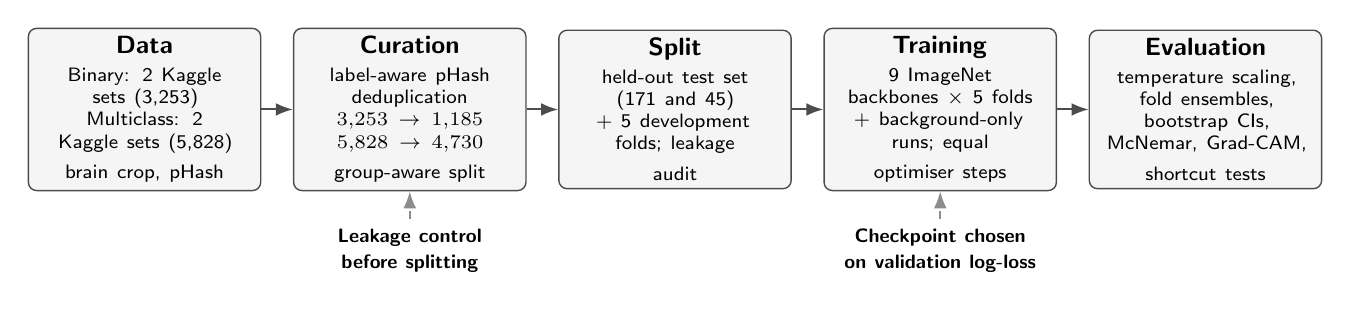
\begin{tikzpicture}[
  font=\sffamily\small,
  >=Latex,
  stage/.style={draw=black!70, fill=black!4, rounded corners=3pt, line width=0.5pt,
                text width=2.74cm, align=center, minimum height=1.75cm, inner sep=3pt},
  lbl/.style={font=\sffamily\bfseries\footnotesize},
  arrow/.style={->, line width=0.7pt, draw=black!70}
]
\node[stage] (acq) {\textbf{Data}\\[2pt]\scriptsize Binary: 2 Kaggle\\ sets (3,253)\\ Multiclass: 2\\ Kaggle sets (5,828)\\ brain crop, pHash};
\node[stage, right=0.4cm of acq] (cur) {\textbf{Curation}\\[2pt]\scriptsize label-aware pHash\\ deduplication\\ $3{,}253\rightarrow1{,}185$\\ $5{,}828\rightarrow4{,}730$\\ group-aware split};
\node[stage, right=0.4cm of cur] (pre) {\textbf{Split}\\[2pt]\scriptsize held-out test set\\ (171 and 45)\\ + 5 development\\ folds; leakage\\ audit};
\node[stage, right=0.4cm of pre] (mod) {\textbf{Training}\\[2pt]\scriptsize 9 ImageNet\\ backbones $\times$ 5 folds\\ + background-only\\ runs; equal\\ optimiser steps};
\node[stage, right=0.4cm of mod] (ev) {\textbf{Evaluation}\\[2pt]\scriptsize temperature scaling,\\ fold ensembles,\\ bootstrap CIs,\\ McNemar, Grad-CAM,\\ shortcut tests};

\draw[arrow] (acq) -- (cur);
\draw[arrow] (cur) -- (pre);
\draw[arrow] (pre) -- (mod);
\draw[arrow] (mod) -- (ev);

\node[below=0.35cm of cur, lbl, text width=3.2cm, align=center] (t1)
  {\scriptsize Leakage control before splitting};
\node[below=0.35cm of mod, lbl, text width=3.2cm, align=center] (t2)
  {\scriptsize Checkpoint chosen on validation log-loss};
\draw[arrow, dashed, draw=black!45] (t1) -- (cur);
\draw[arrow, dashed, draw=black!45] (t2) -- (mod);
\end{tikzpicture}
\caption{Overall methodology of the study. Deduplication and grouping precede every split, so no group of similar images crosses the test set and the development folds. Each backbone is trained on every fold with the same number of optimiser steps, calibrated on its own validation fold, and evaluated on the test set as a five-fold ensemble.}
\label{fig:methodology}
\end{figure*}

\subsection{Data Collection}
\label{sec:data}

For the binary task, which classifies MRI slices as tumour-positive or tumour-negative, two public Kaggle collections were combined. The first, \textit{Brain MRI Images for Brain Tumor Detection} by Chakrabarty \cite{ds1}, contributes 253 images, 155 tumour-positive and 98 tumour-negative. The second, \textit{Br35H: Brain Tumor Detection 2020} \cite{ds2}, contributes 3,000 images, 1,500 of each class. The pooled binary set therefore has 3,253 images, 1,655 tumour-positive and 1,598 tumour-negative. The negative class consists of images that the dataset curators labelled as not containing a tumour; neither source certifies that these images are radiologically normal, so the class is referred to as tumour-negative rather than normal.

For subtype classification into glioma, meningioma and pituitary tumour, two further collections were combined. The first is the \textit{Brain Tumor Classification (MRI)} collection of Bhuvaji et al. \cite{ds3}, whose training and testing folders were merged and whose tumour-negative folder was excluded. The second is the collection of Cheng et al. \cite{ds4}, described in the associated study \cite{ref5}, which comprises 3,064 contrast-enhanced T1-weighted slices from 233 patients and was used in the JPEG conversion distributed on Kaggle \cite{ds5}. The pooled multiclass set has 5,828 images: 2,352 glioma, 1,645 meningioma and 1,831 pituitary.

Table~\ref{tab:provenance} gives the provenance of every image, the native resolution of each source, the share of the image that the brain crop keeps, and the number of images each source lost to deduplication. The binary sources span 184 and 291 distinct image sizes, whereas 99.5\% of the Cheng slices and 93.1\% of the Bhuvaji training folder are $512\times 512$ pixels; the Bhuvaji testing folder is far less uniform, with 184 distinct sizes. Representative images, their brain crops and the head masks used later are shown in Figure~\ref{fig:samples}.

\begin{table*}[htbp]
\centering
\caption{Provenance of the source collections: images per class, native resolution as the number of distinct image sizes and the most common (modal) size with its share, the median fraction of the image kept by the brain crop, and the images removed by deduplication. Bhuvaji removals are recorded for both folders together.}
\label{tab:provenance}
\small
\setlength{\tabcolsep}{3pt}
\begin{tabular*}{\textwidth}{@{\extracolsep{\fill}}llcccccccc@{}}
\toprule
Track & Source & \multicolumn{3}{c}{Images per class} & Total & Sizes & Modal size (share) & Crop kept & Removed \\
\midrule
 & & Tumour & Tumour-neg. & & & & & & \\
\cmidrule(lr){3-4}
\multirow{3}{*}{Binary} & Br35H \cite{ds2} & 1,500 & 1,500 & & 3,000 & 291 & $225\times 225$ (10.9\%) & 0.787 & 2,021 \\
 & Chakrabarty \cite{ds1} & 155 & 98 & & 253 & 184 & $225\times 225$ (7.1\%) & 0.783 & 47 \\
 & \textbf{Total} & \textbf{1,655} & \textbf{1,598} & & \textbf{3,253} & & & & \textbf{2,068} \\
\midrule
 & & Glioma & Meningioma & Pituitary & & & & & \\
\cmidrule(lr){3-5}
\multirow{4}{*}{Multiclass} & Bhuvaji \cite{ds3}, training & 826 & 822 & 827 & 2,475 & 137 & $512\times 512$ (93.1\%) & 0.671 & \multirow{2}{*}{608} \\
 & Bhuvaji \cite{ds3}, testing & 100 & 115 & 74 & 289 & 184 & $512\times 512$ (11.1\%) & 0.846 & \\
 & Cheng \cite{ds4,ds5} & 1,426 & 708 & 930 & 3,064 & 2 & $512\times 512$ (99.5\%) & 0.635 & 486 \\
 & \textbf{Total} & \textbf{2,352} & \textbf{1,645} & \textbf{1,831} & \textbf{5,828} & & & & \textbf{1,094} \\
\bottomrule
\end{tabular*}
\end{table*}

The MRI sequence is unknown in both tracks. Neither binary source records the sequence (T1-weighted, contrast-enhanced T1-weighted, T2-weighted, or FLAIR) of individual images. In the multiclass track, the Cheng component is contrast-enhanced T1-weighted according to its source publication \cite{ref5}, but the Bhuvaji collection records no sequence information, so the pooled multiclass set is a mixture of unknown sequence composition. A model trained on an unknown mixture of sequences cannot be specified for deployment on any particular acquisition protocol. No patient identifiers are available in any source.

\begin{figure*}[htbp]
\centering
\begin{subfigure}{\textwidth}
\centering
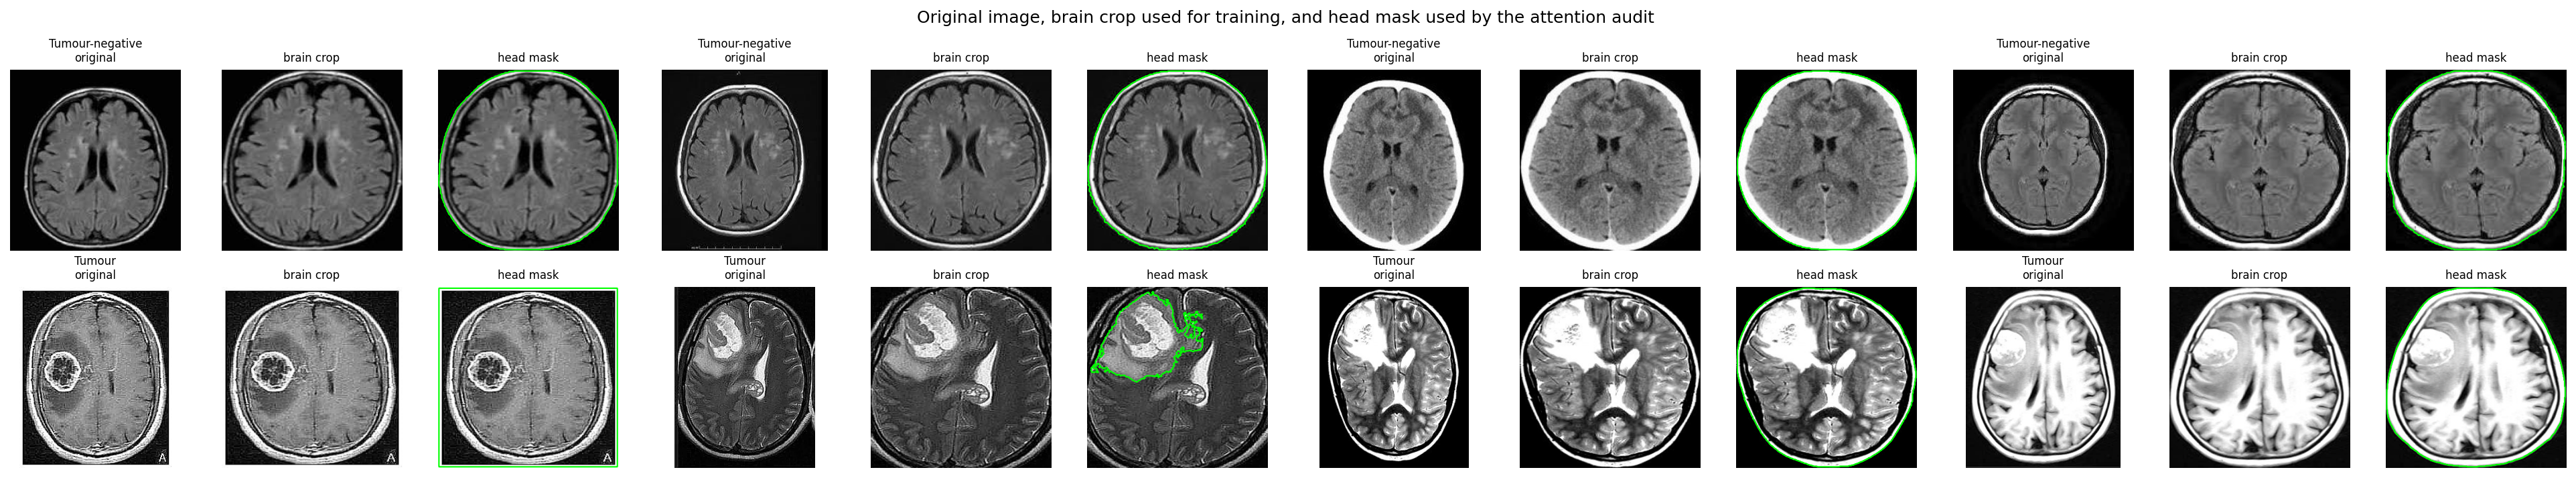
\includegraphics[width=\linewidth]{binary-detection/plots/02_samples_crop_mask.png}
\caption{Binary detection.}
\end{subfigure}
\\[4pt]
\begin{subfigure}{\textwidth}
\centering
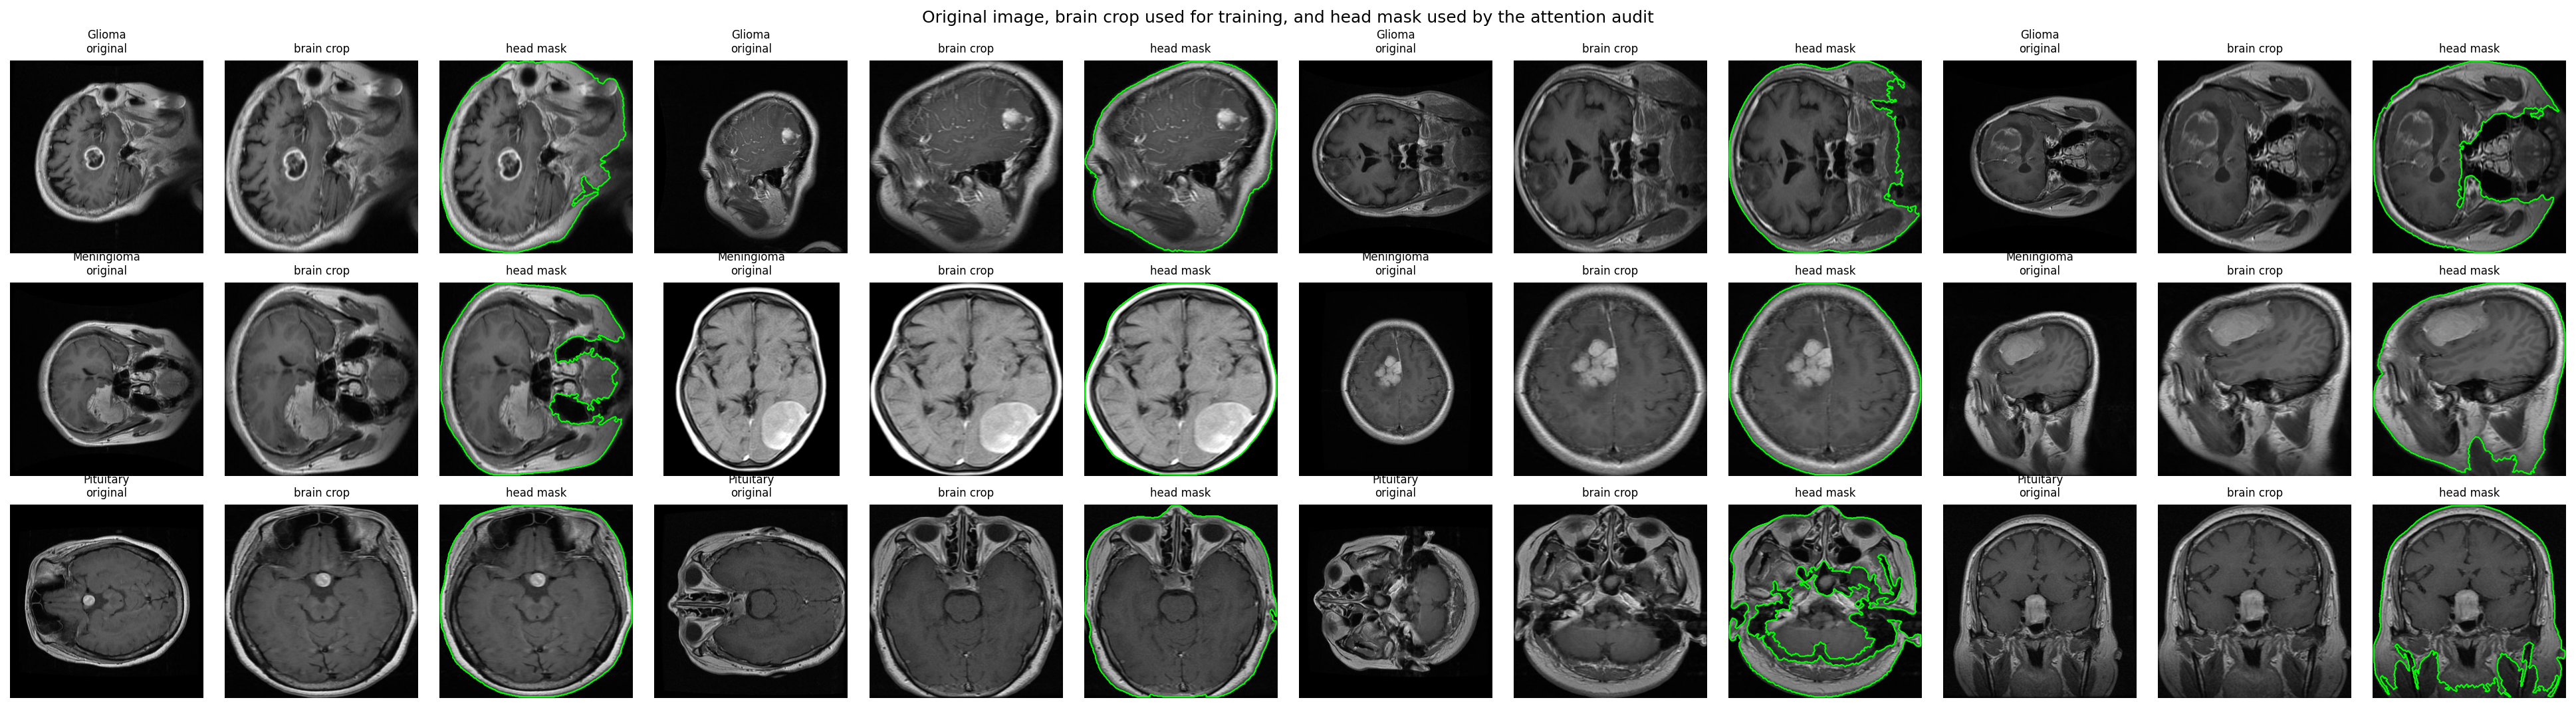
\includegraphics[width=\linewidth]{classification/plots/02_samples_crop_mask.png}
\caption{Subtype classification.}
\end{subfigure}
\caption{Sample images of each class, the brain crop that every model is trained and evaluated on, and the head masks used by the attention and shortcut analyses.}
\label{fig:samples}
\end{figure*}

\subsection{Preprocessing, Deduplication and Splitting}
\label{sec:preproc}

\textbf{Brain crop.} Every image is converted to greyscale, blurred with a $5\times 5$ Gaussian kernel and thresholded at intensity 45, and the bounding box of the largest external contour is kept. This is the crop applied by the web application that deploys the models, so training, evaluation and deployment see the same framing, and it removes most of the empty border around the head. The crops are cached once at $320\times 320$ pixels and resized on the GPU to the input size of each backbone.

\textbf{Label-aware deduplication.} Near-duplicates were identified with 64-bit perceptual hashes computed from the original images: two images within Hamming distance 5 are treated as duplicates, and within each label all but one image of each duplicate set are removed, keeping the copy from the first-listed folder. Pairs within the tolerance that carry different labels were classified with the normalised cross-correlation (NCC) of their $64\times 64$ thumbnails, following the duplicate criterion of Vangala et al. \cite{vangala2026}: at $\mathrm{NCC}\geq 0.98$ the pair is the same image filed under two labels and both copies are excluded as label noise; below that the pair is a hash false positive and both images are kept. The pass ran on each task's pool before any split.

The binary pool contained no cross-label pair within the tolerance. Deduplication removed 2,068 of its 3,253 images (63.57\%), leaving 455 tumour-negative and 730 tumour-positive images (Table~\ref{tab:dedup}). Of the removals, 729 were Br35H images whose retained duplicate is a Chakrabarty image, 1,292 were duplicates within Br35H and 47 within Chakrabarty. In the multiclass pool, 31 cross-label pairs lay within the tolerance, all glioma against meningioma: 8 pairs inside the Bhuvaji collection had NCC of at least 0.9997 and were excluded as label noise, and 23 were hash false positives with NCC between 0.67 and 0.86. Deduplication removed 1,094 multiclass images as duplicates, 608 within Bhuvaji, 483 within Cheng and only 3 Cheng meningioma images against a Bhuvaji copy, and the label-noise exclusion brought the pool to 4,730 images. Per image, the split table records 1,088 duplicates and 10 label-noise exclusions (2 glioma, 8 meningioma); both accounts reach the same 4,730 images. Images kept at other tolerances are listed in Supplementary Table~S1 and plotted in Supplementary Figure~S2, and the multiclass cross-label pairs are shown in Supplementary Figure~S3; tolerances 4 and 5 give the same pool in both tasks.

\begin{table}[htbp]
\centering
\caption{Deduplication outcome per class at Hamming tolerance 5. Label-noise exclusions are those recorded by the per-class summary.}
\label{tab:dedup}
\small
\begin{tabular*}{\textwidth}{@{\extracolsep{\fill}}llccccc@{}}
\toprule
Task & Class & Before & Duplicates & Label noise & After & Removed (\%) \\
\midrule
\multirow{3}{*}{Binary} & Tumour-negative & 1,598 & 1,143 & 0 & 455 & 71.53 \\
 & Tumour & 1,655 & 925 & 0 & 730 & 55.89 \\
 & \textbf{Total} & \textbf{3,253} & \textbf{2,068} & \textbf{0} & \textbf{1,185} & \textbf{63.57} \\
\midrule
\multirow{4}{*}{Multiclass} & Glioma & 2,352 & 342 & 2 & 2,008 & 14.63 \\
 & Meningioma & 1,645 & 329 & 2 & 1,314 & 20.12 \\
 & Pituitary & 1,831 & 423 & 0 & 1,408 & 23.10 \\
 & \textbf{Total} & \textbf{5,828} & \textbf{1,094} & \textbf{4} & \textbf{4,730} & \textbf{18.84} \\
\bottomrule
\end{tabular*}
\end{table}

\textbf{Group-aware split.} Deduplication does not remove correlated but distinct images such as adjacent slices. Kept images within Hamming distance 8 of each other, or with thumbnail $\mathrm{NCC}\geq 0.98$, were therefore joined into groups (connected components), a proxy for patient-level grouping since no source carries patient identifiers. Stratified group $k$-fold sampling then drew a held-out test set of about 15\% of the images and five development folds, so that no group crosses a partition. A leakage audit measured, for every test image, the nearest development image by Hamming distance and NCC: in both tasks no test image has a development image within Hamming distance 5, within distance 8, or at $\mathrm{NCC}\geq 0.98$ (Supplementary Figure~S4).

The binary pool formed 821 groups, the largest of 7 images, and the split gave 1,014 development images in folds of 184 to 211 images and a test set of 171 images (107 tumour, 64 tumour-negative; Table~\ref{tab:splits}). The multiclass pool formed 1,867 groups, but one of them held 1,431 images, more than 5\% of the pool, and the notebook warned that a smaller grouping tolerance should be considered. The run kept the tolerance of 8. Because a group cannot be divided, the multiclass split is highly uneven: the development folds hold 154 to 2,216 images, and the held-out test set holds only 45 images, of which 1 is glioma, 13 meningioma and 31 pituitary. The multiclass test results in Section~\ref{sec:multiclass-results} must be read with this in mind.

\begin{table}[htbp]
\centering
\caption{Images per partition after deduplication and grouping. Development images are divided into five group-aware folds; fold sizes are given in the last column.}
\label{tab:splits}
\small
\begin{tabular*}{\textwidth}{@{\extracolsep{\fill}}llccl@{}}
\toprule
Task & Class & Development & Test & Fold sizes (0--4) \\
\midrule
\multirow{3}{*}{Binary} & Tumour-negative & 391 & 64 & \\
 & Tumour & 623 & 107 & \\
 & \textbf{Total} & \textbf{1,014} & \textbf{171} & 184, 211, 207, 210, 202 \\
\midrule
\multirow{4}{*}{Multiclass} & Glioma & 2,007 & 1 & \\
 & Meningioma & 1,301 & 13 & \\
 & Pituitary & 1,377 & 31 & \\
 & \textbf{Total} & \textbf{4,685} & \textbf{45} & 154, 742, 697, 876, 2,216 \\
\bottomrule
\end{tabular*}
\end{table}

\textbf{Normalisation and augmentation.} Crops are scaled to $[0,1]$ and normalised with the ImageNet channel means of $[0.485, 0.456, 0.406]$ and standard deviations of $[0.229, 0.224, 0.225]$. Training augmentation runs on the GPU and consists of horizontal flipping with probability 0.5, rotation of up to $\pm 10$ degrees, and brightness and contrast jitter of up to 20\%; validation and test images are not augmented. Examples are shown in Supplementary Figure~S5, and the dataset overviews in Supplementary Figure~S1.

\subsection{Model Development}
\label{sec:models}

Nine architectures spanning three families were evaluated, all built from one model registry so that a model name means the same implementation and the same pretrained checkpoint in both tasks. Eight are \texttt{torchvision} models loaded with their default ImageNet weights, and CoAtNet-0 is the \texttt{timm} model \texttt{coatnet\_0\_rw\_224}, since CoAtNet has no \texttt{torchvision} implementation. In every model the final linear layer is replaced by one with one output for the binary task or three for the multiclass task. The auxiliary classifier of InceptionV3 is removed, so no model receives an extra loss term and no unused parameters are counted.

ResNet50 is a 50-layer residual network built around bottleneck residual blocks with skip connections, with 23.51 million parameters in the binary configuration. VGG16 stacks $3\times 3$ convolutions in increasing depth and has 134.26 million parameters. DenseNet121 concatenates the feature maps of all preceding layers within each dense block and has 6.95 million parameters. EfficientNetB0, developed through neural architecture search and compound scaling, has 4.01 million parameters and needs 0.77 GFLOPs per image. MobileNetV3-Large uses depth-wise separable convolutions for mobile devices and has 4.20 million parameters and the lowest cost in the study, 0.43 GFLOPs. InceptionV3 uses parallel convolutional paths of different kernel sizes, has 21.79 million parameters, and is the only model run at its native $299\times 299$ input, at which it needs 11.42 GFLOPs against 5.67 GFLOPs at $224\times 224$. ViT-B/16 processes $16\times 16$ patches as a token sequence with a transformer encoder and has 85.80 million parameters. Swin-Base uses hierarchical shifted-window attention and has 86.74 million parameters. CoAtNet-0 combines convolutional and attention stages and has 26.67 million parameters. The multiclass heads add a few thousand parameters to each count (for example 4.011 million for EfficientNetB0 and 134.27 million for VGG16). Parameter counts and GFLOPs are those measured by the notebook on the instantiated models and are listed in Table~\ref{tab:efficiency}.

\subsection{Training Configuration}
\label{sec:training}

All experiments ran on Kaggle with two NVIDIA Tesla T4 graphics processing units, four central processing unit cores and 33.7~GB of system memory, using Python 3.13.15, PyTorch 2.11.0, torchvision 0.26.0, timm 1.0.29 and CUDA 12.8. Two worker processes, one per GPU, trained different (model, fold) jobs in parallel. The settings in Table~\ref{tab:hyperparams} were identical for every model and both tasks.

Every model used the same effective batch of 64 images and 20 epochs. The largest micro-batch that fitted on one GPU was probed for each model, and gradient accumulation made up the difference: Swin-Base trained with micro-batches of 32 accumulated over two steps, every other model with micro-batches of 64. All models therefore receive the same number of optimiser steps on the same fold: 260 steps for every binary run (13 steps per epoch), and 1,420, 1,240, 1,260, 1,200 and 780 steps on multiclass folds 0 to 4, whose training sets differ in size because of the uneven split. Every training image is used in every epoch. The optimiser was AdamW with a learning rate of $3\times 10^{-4}$ and weight decay 0.01, with a linear warm-up over the first epoch followed by cosine decay applied per optimiser step, half-precision autocasting with gradient scaling, and gradient clipping at a norm of 1.0. The loss was binary cross-entropy with logits for detection and cross-entropy for subtypes. After every epoch the validation fold was evaluated, and the checkpoint with the lowest validation log-loss, a continuous proper scoring rule, was kept.

For the shortcut test of Section~\ref{sec:interpretability}, each backbone was also trained once on fold 0 with the head region of every image set to zero, so that only background, borders and framing remain. With 45 full-image runs and 9 background-only runs per task, each notebook trained 54 jobs; all 54 finished in both tasks, in 63.5 minutes of training for detection and 264.6 minutes for subtypes. The random seed was 42; deterministic kernels were not enforced, so re-running the notebooks should reproduce the reported figures closely but not necessarily bit for bit.

\begin{table}[htbp]
\centering
\caption{Training settings, identical for all nine models and both tasks.}
\label{tab:hyperparams}
\small
\begin{tabularx}{\textwidth}{@{}lY@{}}
\toprule
Setting & Value \\
\midrule
Epochs & 20, with 1 warm-up epoch \\
Effective batch & 64 images, through gradient accumulation \\
Optimiser steps & Equal for every model on a given fold (binary 260; multiclass 780 to 1,420 by fold) \\
Optimiser & AdamW, learning rate $3\times 10^{-4}$, weight decay 0.01 \\
Learning rate schedule & Linear warm-up, then cosine decay per optimiser step \\
Loss & Binary cross-entropy with logits (detection); cross-entropy (subtypes) \\
Precision & Half-precision autocasting with gradient scaling \\
Gradient clipping & Norm 1.0 \\
Input resolution & $224\times 224$ pixels; $299\times 299$ pixels for InceptionV3 \\
Augmentation & Horizontal flip ($p=0.5$), rotation up to $\pm 10^{\circ}$, brightness and contrast jitter of 20\% \\
Checkpoint selection & Lowest validation log-loss \\
Cross-validation & 5 group-aware folds plus a fixed held-out test set \\
Random seed & 42 \\
\bottomrule
\end{tabularx}
\end{table}

\subsection{Evaluation Protocol}
\label{sec:evaluation}

\textbf{Calibration and thresholds.} For every run, a temperature was fitted on its own validation fold by minimising the negative log-likelihood \cite{guo2017}, searching $\log T$ in $[-3, 3]$, and applied to its test logits. For binary runs, a decision threshold was also chosen on the validation fold by Youden's J statistic. The expected calibration error (ECE) uses 15 equal-width confidence bins.

\textbf{Cross-validation and fold ensembles.} Each run is scored on the held-out test set, and the five runs of each backbone are summarised as mean and standard deviation. For the headline comparison, the calibrated test probabilities of the five folds are averaged into one fold-ensemble prediction per image. Accuracy, macro F1 and area under the receiver operating characteristic curve (AUC) receive percentile bootstrap 95\% confidence intervals from 2,000 resamples of the test images. Binary sensitivity and specificity are reported at a threshold of 0.5 and at the mean validation-tuned threshold.

\textbf{Statistical comparison.} Every pair of fold ensembles was compared with an exact McNemar test, and the p-values were adjusted with the Holm procedure \cite{holm1979}. For each model, the bootstrap 95\% confidence interval of its accuracy gap to the leading model was also computed; a model whose interval includes zero cannot be separated from the leader on this test set. Test accuracy was further broken down by the Hamming distance from each test image to its nearest development image.

\textbf{Attention and shortcut analysis.} For each backbone, the fold with the lowest validation loss was reloaded and gradient-weighted class activation maps (Grad-CAM) \cite{selvaraju2017} were computed for every test image at the last spatial or token stage of the network; for VGG16 this is the last convolution. ViT-B/16 additionally received attention rollout \cite{abnar2020}. A head mask was computed for every image by Otsu thresholding, morphological closing, selection of the largest connected component and hole filling, and the share of map energy outside the mask was compared with the share a uniform map would give. Because Grad-CAM maps of convolutional and attention stages are not strictly commensurable, occlusion sensitivity, the drop in predicted-class probability when a $32\times 32$ patch moved with stride 16 is replaced by the image mean, was computed in the same way for every model on a common stratified sample of test images. An inference-only masking test applied each fold's checkpoint to test images with the head set to zero or the background set to zero. Finally, the background-only models of Section~\ref{sec:training} were tested on background-only test images; accuracy significantly above the majority-class rate, by a one-sided exact binomial test with Holm correction, shows that the background carries label information a model can exploit.

\textbf{Efficiency.} After training, each model was timed on one T4 with no other work on the device, under half-precision autocasting: single-image latency over 100 passes after 10 warm-up passes, and throughput at batch size 32 over 20 passes after 3 warm-up passes, with the whole protocol repeated three times. Training time, training throughput and peak training memory are averaged over the folds; because the two workers shared four CPU cores, training throughput is a lower bound.

\section{Results and Discussion}
\label{sec:results}

Section~\ref{sec:cv-results} reports cross-validation, Sections~\ref{sec:binary-results} and \ref{sec:multiclass-results} the fold-ensemble test results of each task, Section~\ref{sec:calibration} calibration, Section~\ref{sec:efficiency} efficiency, Section~\ref{sec:interpretability} attention and shortcut analyses, and Section~\ref{sec:comparison} the comparison with published work.

\subsection{Cross-Validation Results}
\label{sec:cv-results}

Table~\ref{tab:cv} summarises the test accuracy, macro F1 and AUC of the individual fold models. In binary detection, mean accuracy ranges from 95.91\% for VGG16 to 97.89\% for InceptionV3, and the standard deviations across folds, from 0.32 to 2.20 percentage points, are of the same size as most gaps between neighbouring models. The fold models disagree more with each other than the backbones do on average: CoAtNet-0, for example, scores between 94.74\% and 98.83\% on its five folds. In subtype classification, every model averages between 97.33\% and 99.56\%, but each fold model is scored on the same 45 test images, so one image changes accuracy by 2.22 percentage points. Training curves for all models are given in Supplementary Figures~S6 and S7, and the temperature, threshold and test result of every run in Supplementary Tables~S2 and S3.

\begin{table*}[htbp]
\centering
\caption{Test results of the individual fold models: mean $\pm$ standard deviation over the five folds of each backbone, after temperature scaling. Binary detection is evaluated on 171 test images and subtype classification on 45. Rows are ordered by binary accuracy.}
\label{tab:cv}
\small
\begin{tabular*}{\textwidth}{@{\extracolsep{\fill}}lcccccc@{}}
\toprule
 & \multicolumn{3}{c}{Binary detection} & \multicolumn{3}{c}{Subtype classification} \\
\cmidrule(lr){2-4}\cmidrule(l){5-7}
Model & Accuracy (\%) & Macro F1 (\%) & AUC & Accuracy (\%) & Macro F1 (\%) & AUC \\
\midrule
InceptionV3 & $97.89\pm 0.32$ & $97.75\pm 0.34$ & $0.9966\pm 0.0042$ & $99.56\pm 0.99$ & $97.51\pm 5.57$ & $1.0000\pm 0.0000$ \\
Swin-Base & $97.78\pm 1.62$ & $97.64\pm 1.72$ & $0.9974\pm 0.0026$ & $99.56\pm 0.99$ & $97.51\pm 5.57$ & $1.0000\pm 0.0000$ \\
EfficientNetB0 & $97.78\pm 0.49$ & $97.62\pm 0.52$ & $0.9968\pm 0.0034$ & $97.33\pm 3.65$ & $90.61\pm 9.43$ & $0.9989\pm 0.0017$ \\
CoAtNet-0 & $97.54\pm 1.72$ & $97.39\pm 1.83$ & $0.9966\pm 0.0038$ & $98.67\pm 1.22$ & $94.67\pm 6.53$ & $1.0000\pm 0.0000$ \\
ViT-B/16 & $97.54\pm 0.96$ & $97.37\pm 1.04$ & $0.9970\pm 0.0013$ & $99.11\pm 1.22$ & $95.02\pm 6.82$ & $0.9995\pm 0.0011$ \\
DenseNet121 & $97.19\pm 0.76$ & $96.98\pm 0.82$ & $0.9927\pm 0.0048$ & $99.11\pm 1.22$ & $97.15\pm 5.42$ & $0.9998\pm 0.0004$ \\
ResNet50 & $96.84\pm 1.35$ & $96.60\pm 1.46$ & $0.9876\pm 0.0105$ & $98.67\pm 1.22$ & $92.69\pm 6.68$ & $0.9998\pm 0.0004$ \\
MobileNetV3-Large & $96.37\pm 2.20$ & $96.16\pm 2.30$ & $0.9946\pm 0.0033$ & $97.78\pm 0.00$ & $87.56\pm 0.00$ & $0.9998\pm 0.0004$ \\
VGG16 & $95.91\pm 0.83$ & $95.65\pm 0.88$ & $0.9943\pm 0.0023$ & $97.33\pm 2.43$ & $88.46\pm 7.30$ & $0.9989\pm 0.0021$ \\
\bottomrule
\end{tabular*}
\end{table*}

\subsection{Binary Detection Results}
\label{sec:binary-results}

Table~\ref{tab:binary-results} reports the fold ensembles on the 171 binary test images, and Supplementary Table~S4 the per-class metrics. CoAtNet-0, EfficientNetB0 and ViT-B/16 each misclassified one image, an accuracy of 99.42\% with a bootstrap 95\% confidence interval of 98.25\% to 100\%. Their single errors differ in kind: CoAtNet-0 missed one tumour, whereas EfficientNetB0 and ViT-B/16 detected every tumour and raised one false alarm. Swin-Base followed at 98.83\% with two missed tumours, then InceptionV3 and ResNet50 at 98.25\%, and DenseNet121, MobileNetV3-Large and VGG16 at 97.08\%. Every AUC lies between 0.9974 and 0.9997. The confusion matrices of all nine ensembles are shown in Figure~\ref{fig:binary-confusion}, and the receiver operating characteristic and precision--recall curves in Supplementary Figure~S8.

These differences are small relative to the test set. No pair of models differs significantly by the exact McNemar test after Holm correction: every adjusted p-value is 1.0 (Supplementary Figure~S9). The bootstrap interval of the accuracy gap to CoAtNet-0 excludes zero only for VGG16 and MobileNetV3-Large, both 2.34 percentage points behind with an interval of 0.58 to 4.68 points; ResNet50, InceptionV3, DenseNet121, Swin-Base, EfficientNetB0 and ViT-B/16 cannot be separated from the leader. Accuracy also does not fall for test images that are furthest from the development pool: with nearest development images at Hamming distance 17 to 20, every model is correct on every image (Supplementary Table~S5).

At the mean validation-tuned thresholds, which range from 0.43 to 0.84, accuracy is between 96.49\% and 98.83\%, and for EfficientNetB0 sensitivity falls from 100\% to 96.26\% while specificity stays at 98.44\%. The tuned thresholds raise accuracy only for DenseNet121 (97.66\% against 97.08\%), leave it unchanged for InceptionV3 and VGG16, and lower it for the other six models.

\begin{table*}[htbp]
\centering
\caption{Binary detection: fold ensembles on the 171 held-out test images (107 tumour, 64 tumour-negative). Sensitivity is recall of the tumour class and specificity recall of the tumour-negative class, both at threshold 0.5; FN and FP are missed tumours and false alarms. Accuracy has a bootstrap 95\% confidence interval. Rows are ordered by accuracy.}
\label{tab:binary-results}
\small
\begin{tabular*}{\textwidth}{@{\extracolsep{\fill}}lcccccccc@{}}
\toprule
Model & Accuracy (\%) [95\% CI] & Bal. acc. (\%) & Sens. (\%) & Spec. (\%) & MCC & AUC & FN & FP \\
\midrule
CoAtNet-0 & 99.42 [98.25, 100] & 99.53 & 99.07 & 100.00 & 0.9876 & 0.9994 & 1 & 0 \\
EfficientNetB0 & 99.42 [98.25, 100] & 99.22 & 100.00 & 98.44 & 0.9876 & 0.9991 & 0 & 1 \\
ViT-B/16 & 99.42 [98.25, 100] & 99.22 & 100.00 & 98.44 & 0.9876 & 0.9984 & 0 & 1 \\
Swin-Base & 98.83 [97.08, 100] & 99.07 & 98.13 & 100.00 & 0.9755 & 0.9997 & 2 & 0 \\
InceptionV3 & 98.25 [95.91, 100] & 97.97 & 99.07 & 96.88 & 0.9625 & 0.9991 & 1 & 2 \\
ResNet50 & 98.25 [95.91, 100] & 98.28 & 98.13 & 98.44 & 0.9627 & 0.9988 & 2 & 1 \\
DenseNet121 & 97.08 [94.15, 99.42] & 96.41 & 99.07 & 93.75 & 0.9376 & 0.9984 & 1 & 4 \\
MobileNetV3-Large & 97.08 [94.15, 99.42] & 97.04 & 97.20 & 96.88 & 0.9378 & 0.9978 & 3 & 2 \\
VGG16 & 97.08 [94.15, 99.42] & 97.04 & 97.20 & 96.88 & 0.9378 & 0.9974 & 3 & 2 \\
\bottomrule
\end{tabular*}
\end{table*}

\begin{figure*}[htbp]
\centering
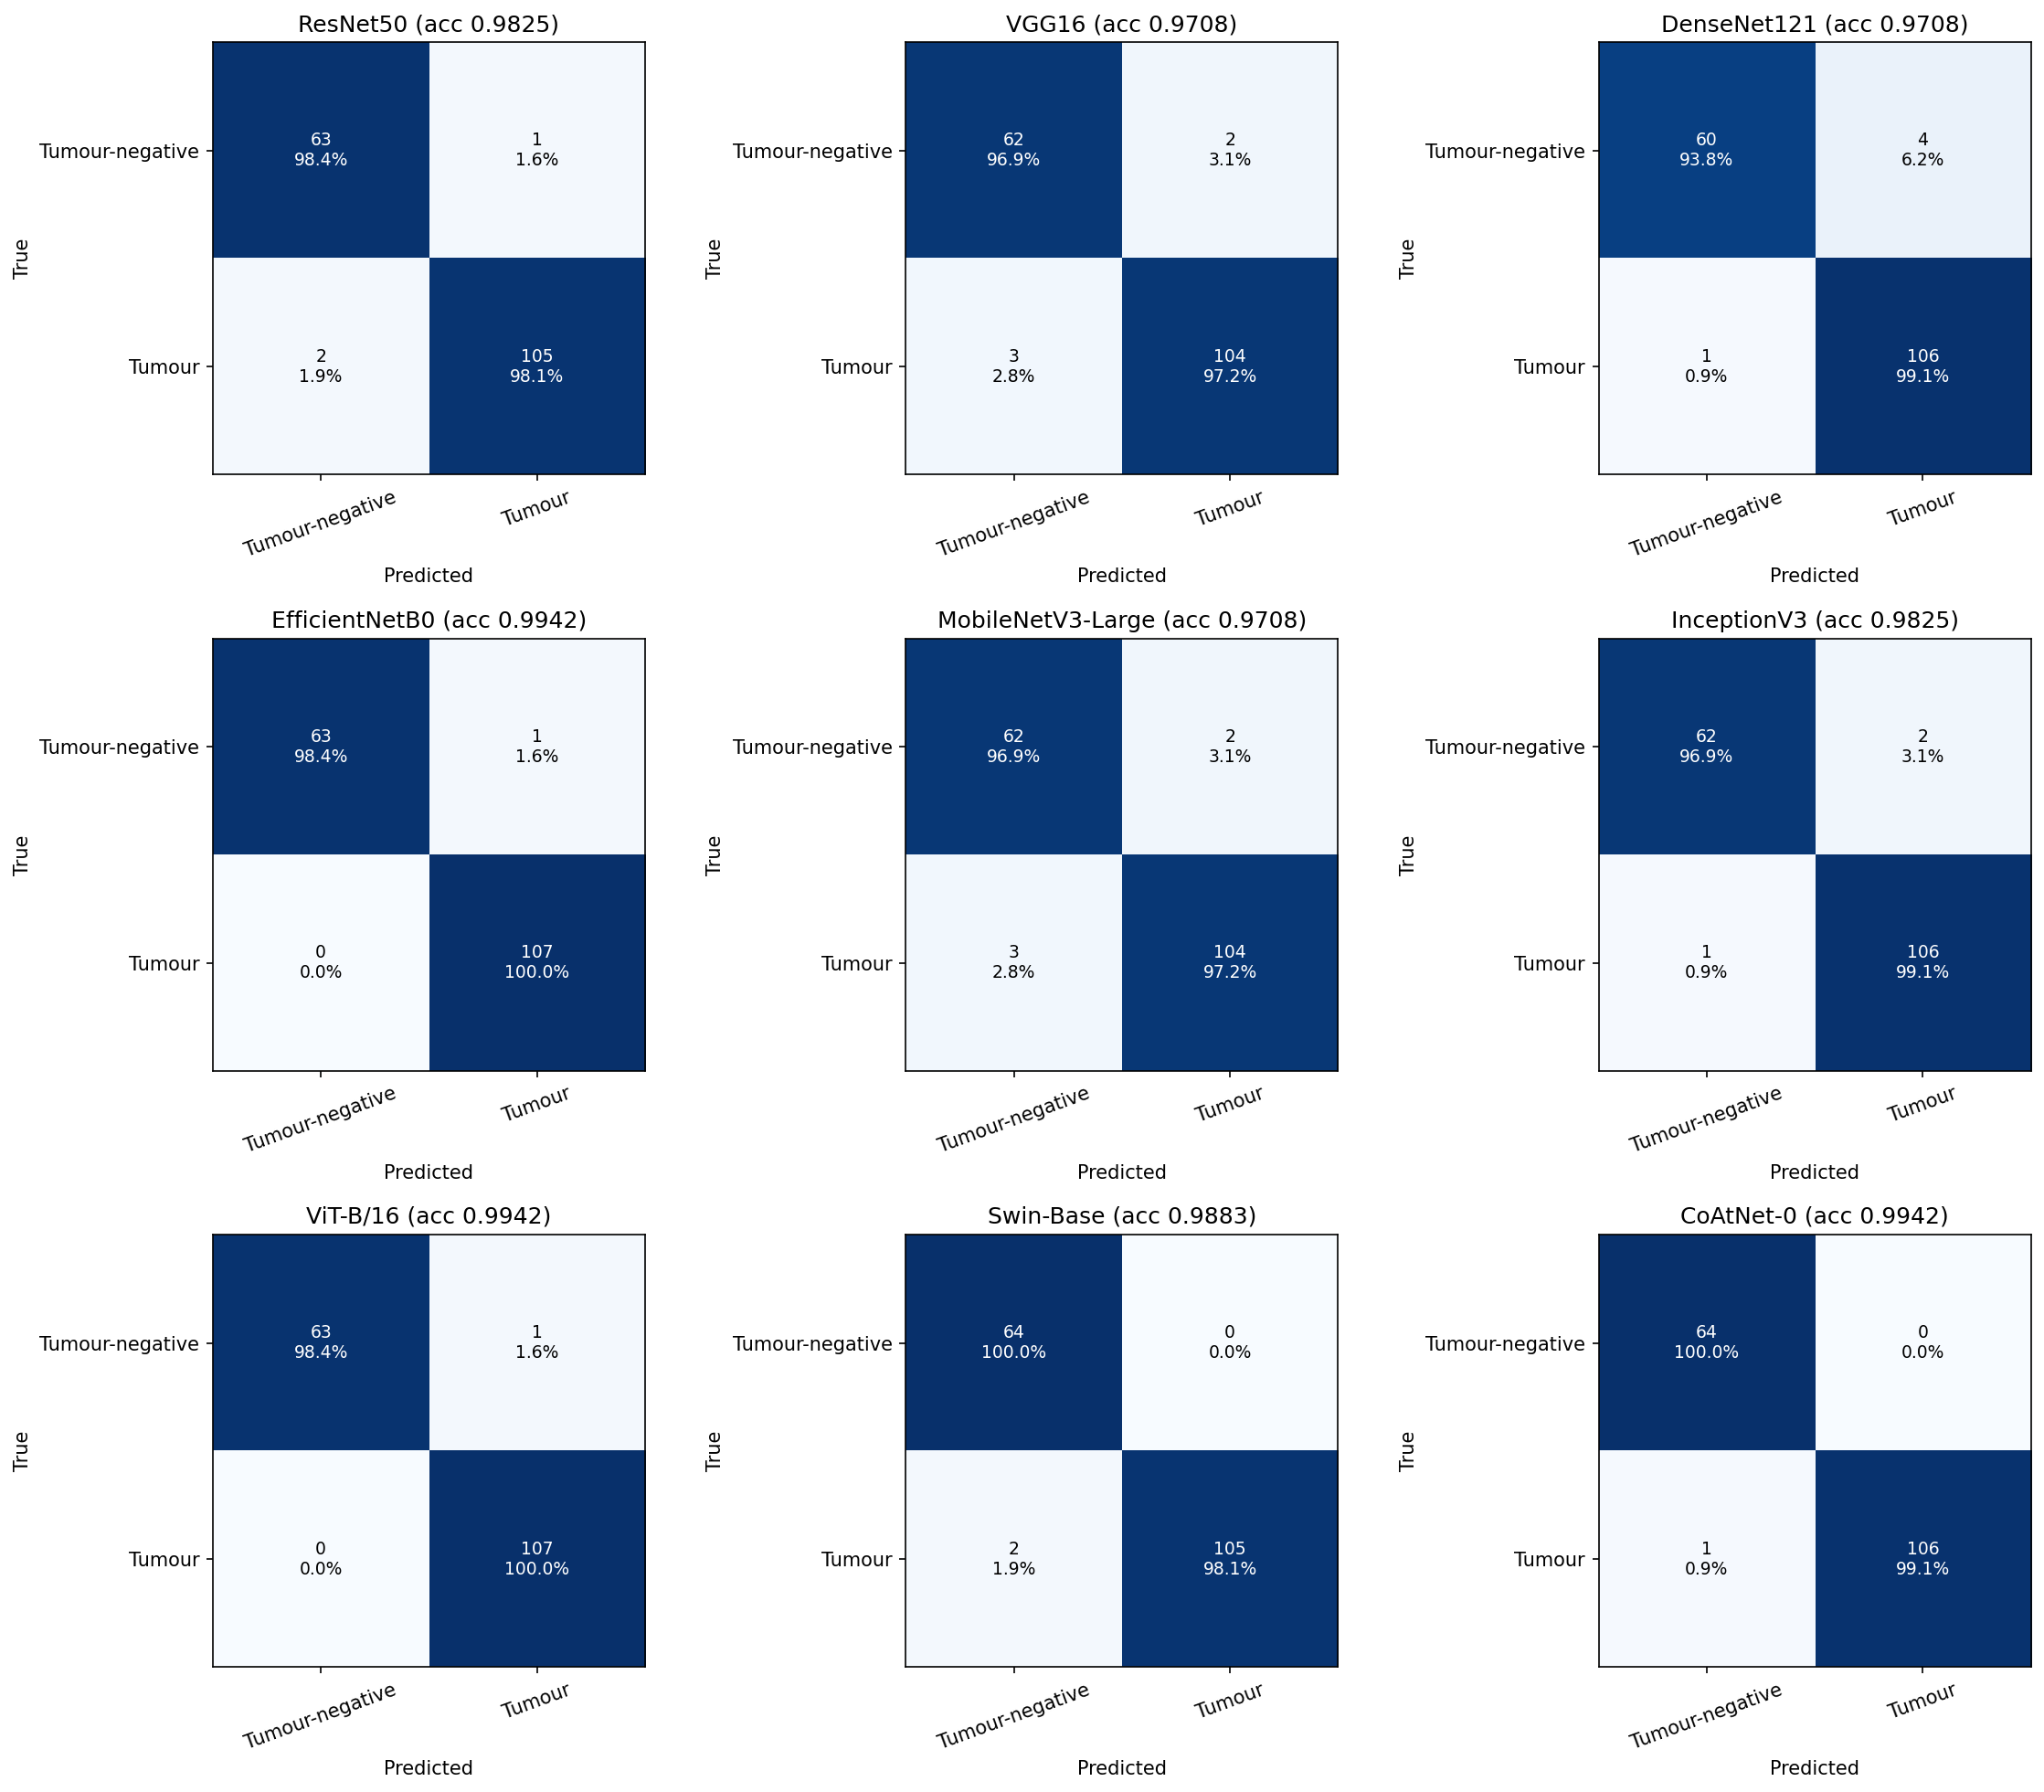
\includegraphics[width=\linewidth]{binary-detection/plots/09_confusion_matrices.png}
\caption{Binary detection: test confusion matrices of the fold ensemble of every model, as counts with row percentages.}
\label{fig:binary-confusion}
\end{figure*}

\subsection{Subtype Classification Results}
\label{sec:multiclass-results}

Table~\ref{tab:multiclass-results} reports the fold ensembles on the 45 multiclass test images. ResNet50, DenseNet121, InceptionV3, ViT-B/16, Swin-Base and CoAtNet-0 classified every image correctly. VGG16, EfficientNetB0 and MobileNetV3-Large made the same single error, a meningioma image predicted as glioma, for an accuracy of 97.78\%; because the test set contains only one glioma image, that error halves glioma precision and pulls macro F1 down to 87.56\%. Every model reaches an AUC of 1.0, no McNemar comparison is significant, and every bootstrap interval of the gap to the leader includes zero. The confusion matrices are shown in Supplementary Figure~S10.

This test set cannot rank the models. It contains 45 images, one of them glioma, because a single group of 1,431 images could not be divided between partitions (Section~\ref{sec:preproc}); its class balance (2.2\% glioma, 28.9\% meningioma, 68.9\% pituitary) is far from that of the pool. The cross-validation results in Table~\ref{tab:cv} are scored on the same 45 images and inherit the same limitation. The multiclass results therefore show that every backbone separates these subtypes on images that are not near-copies of its training images, but they do not establish an ordering of the backbones, and the 100\% accuracies should not be quoted as an estimate of subtype accuracy in general.

\begin{table}[htbp]
\centering
\caption{Subtype classification: fold ensembles on the 45 held-out test images (1 glioma, 13 meningioma, 31 pituitary). Precision and F1 are macro-averaged; AUC is the macro one-versus-rest value. Accuracy has a bootstrap 95\% confidence interval.}
\label{tab:multiclass-results}
\small
\begin{tabular*}{\textwidth}{@{\extracolsep{\fill}}lcccccc@{}}
\toprule
Model & Accuracy (\%) [95\% CI] & Bal. acc. (\%) & Prec. (\%) & F1 (\%) & MCC & AUC \\
\midrule
ResNet50 & 100.00 [100, 100] & 100.00 & 100.00 & 100.00 & 1.0000 & 1.0000 \\
DenseNet121 & 100.00 [100, 100] & 100.00 & 100.00 & 100.00 & 1.0000 & 1.0000 \\
InceptionV3 & 100.00 [100, 100] & 100.00 & 100.00 & 100.00 & 1.0000 & 1.0000 \\
ViT-B/16 & 100.00 [100, 100] & 100.00 & 100.00 & 100.00 & 1.0000 & 1.0000 \\
Swin-Base & 100.00 [100, 100] & 100.00 & 100.00 & 100.00 & 1.0000 & 1.0000 \\
CoAtNet-0 & 100.00 [100, 100] & 100.00 & 100.00 & 100.00 & 1.0000 & 1.0000 \\
VGG16 & 97.78 [93.33, 100] & 97.44 & 83.33 & 87.56 & 0.9515 & 1.0000 \\
EfficientNetB0 & 97.78 [93.33, 100] & 97.44 & 83.33 & 87.56 & 0.9515 & 1.0000 \\
MobileNetV3-Large & 97.78 [93.33, 100] & 97.44 & 83.33 & 87.56 & 0.9515 & 1.0000 \\
\bottomrule
\end{tabular*}
\end{table}

\subsection{Calibration}
\label{sec:calibration}

Table~\ref{tab:calibration} gives the ECE of the fold ensembles before and after temperature scaling. Every model is reasonably calibrated, with ECE between 0.0146 and 0.0326 in detection and between 0.0044 and 0.0371 in classification. Temperature scaling, however, lowered the ECE only for ResNet50 and ViT-B/16 in detection and for CoAtNet-0 in classification, and raised it for every other model. The cause is visible in the per-run temperatures (Supplementary Tables~S2 and S3): when a validation fold is classified almost perfectly, minimising its negative log-likelihood drives the temperature towards the lower bound of the search, $e^{-3}\approx 0.0498$, which sharpens the test probabilities. In binary fold 4 the fitted temperature of six models lies between 0.0498 and 0.0682, and for five of them that fold has the highest test log-loss of the model's five folds, for example 0.543 for EfficientNetB0 against 0.038 to 0.088 on its other folds. Validation folds of a few hundred near-separable images are too small to fit a temperature reliably. Reliability diagrams are given in Supplementary Figure~S11.

\begin{table}[htbp]
\centering
\caption{Expected calibration error of the fold ensembles on the held-out test set, after and before temperature scaling.}
\label{tab:calibration}
\small
\begin{tabular*}{\textwidth}{@{\extracolsep{\fill}}lcccc@{}}
\toprule
 & \multicolumn{2}{c}{Binary detection} & \multicolumn{2}{c}{Subtype classification} \\
\cmidrule(lr){2-3}\cmidrule(l){4-5}
Model & Scaled & Uncalibrated & Scaled & Uncalibrated \\
\midrule
CoAtNet-0 & 0.0275 & 0.0207 & 0.0253 & 0.0259 \\
DenseNet121 & 0.0252 & 0.0233 & 0.0215 & 0.0165 \\
EfficientNetB0 & 0.0243 & 0.0231 & 0.0277 & 0.0263 \\
InceptionV3 & 0.0228 & 0.0151 & 0.0088 & 0.0045 \\
MobileNetV3-Large & 0.0326 & 0.0146 & 0.0285 & 0.0204 \\
ResNet50 & 0.0157 & 0.0173 & 0.0222 & 0.0125 \\
Swin-Base & 0.0152 & 0.0148 & 0.0109 & 0.0044 \\
VGG16 & 0.0296 & 0.0179 & 0.0371 & 0.0355 \\
ViT-B/16 & 0.0207 & 0.0222 & 0.0182 & 0.0114 \\
\bottomrule
\end{tabular*}
\end{table}

\subsection{Model Efficiency Comparison}
\label{sec:efficiency}

Table~\ref{tab:efficiency} compares the cost of the nine backbones. Cost varies by more than two orders of magnitude, from 0.43 GFLOPs for MobileNetV3-Large to 30.9 GFLOPs for Swin-Base and VGG16, while binary test accuracy varies by 2.34 percentage points and the differences are not significant. MobileNetV3-Large has the highest batched throughput, 2,301 images per second in detection, and EfficientNetB0 follows at 1,393 images per second with an accuracy equal to the leaders; Swin-Base has the lowest throughput at 198 images per second and the highest single-image latency at 36.3~ms. Single-image latency does not follow model size: VGG16, the largest model, has the lowest latency at 7.7~ms in detection and 8.0~ms in classification, whereas DenseNet121 needs 23.6~ms and 22.8~ms despite its 6.95 million parameters, so neither parameter count nor GFLOPs predicts single-image latency on this hardware. Peak training memory ranges from 2.1~GB for MobileNetV3-Large to 11.4~GB for CoAtNet-0. Accuracy is plotted against latency in Figure~\ref{fig:latency} and Supplementary Figure~S13; the full measurements, including standard deviations and training throughput, are in Supplementary Table~S6.

\begin{table*}[htbp]
\centering
\caption{Computational cost of the nine backbones. Parameters and GFLOPs are measured on the binary models at the native input ($299\times 299$ for InceptionV3, which needs 5.67 GFLOPs at $224\times 224$). Latency is the mean of single-image passes and throughput the mean at batch size 32, both on one Tesla T4 under half-precision autocasting and pooled over three repeats. Training time is minutes per run, averaged over folds. Rows are ordered by parameter count.}
\label{tab:efficiency}
\small
\begin{tabular*}{\textwidth}{@{\extracolsep{\fill}}lcccccccc@{}}
\toprule
 & & & \multicolumn{2}{c}{Latency (ms)} & \multicolumn{2}{c}{Throughput (img/s)} & \multicolumn{2}{c}{Training (min/run)} \\
\cmidrule(lr){4-5}\cmidrule(lr){6-7}\cmidrule(l){8-9}
Model & Params (M) & GFLOPs & Bin. & Multi. & Bin. & Multi. & Bin. & Multi. \\
\midrule
EfficientNetB0 & 4.01 & 0.77 & 13.1 & 12.8 & 1,393 & 1,266 & 2.0 & 5.1 \\
MobileNetV3-Large & 4.20 & 0.43 & 10.6 & 10.0 & 2,301 & 2,183 & 1.5 & 3.5 \\
DenseNet121 & 6.95 & 5.67 & 23.6 & 22.8 & 657 & 608 & 1.5 & 6.9 \\
InceptionV3 & 21.79 & 11.42 & 17.6 & 16.7 & 512 & 438 & 1.7 & 8.0 \\
ResNet50 & 23.51 & 8.17 & 9.6 & 9.1 & 777 & 717 & 1.2 & 5.3 \\
CoAtNet-0 & 26.67 & 8.42 & 16.5 & 15.9 & 513 & 448 & 2.3 & 9.5 \\
ViT-B/16 & 85.80 & 22.54 & 11.0 & 10.3 & 272 & 241 & 2.9 & 15.0 \\
Swin-Base & 86.74 & 30.86 & 36.3 & 34.6 & 198 & 173 & 4.3 & 21.4 \\
VGG16 & 134.26 & 30.93 & 7.7 & 8.0 & 386 & 332 & 2.2 & 9.5 \\
\bottomrule
\end{tabular*}
\end{table*}

\begin{figure}[htbp]
\centering
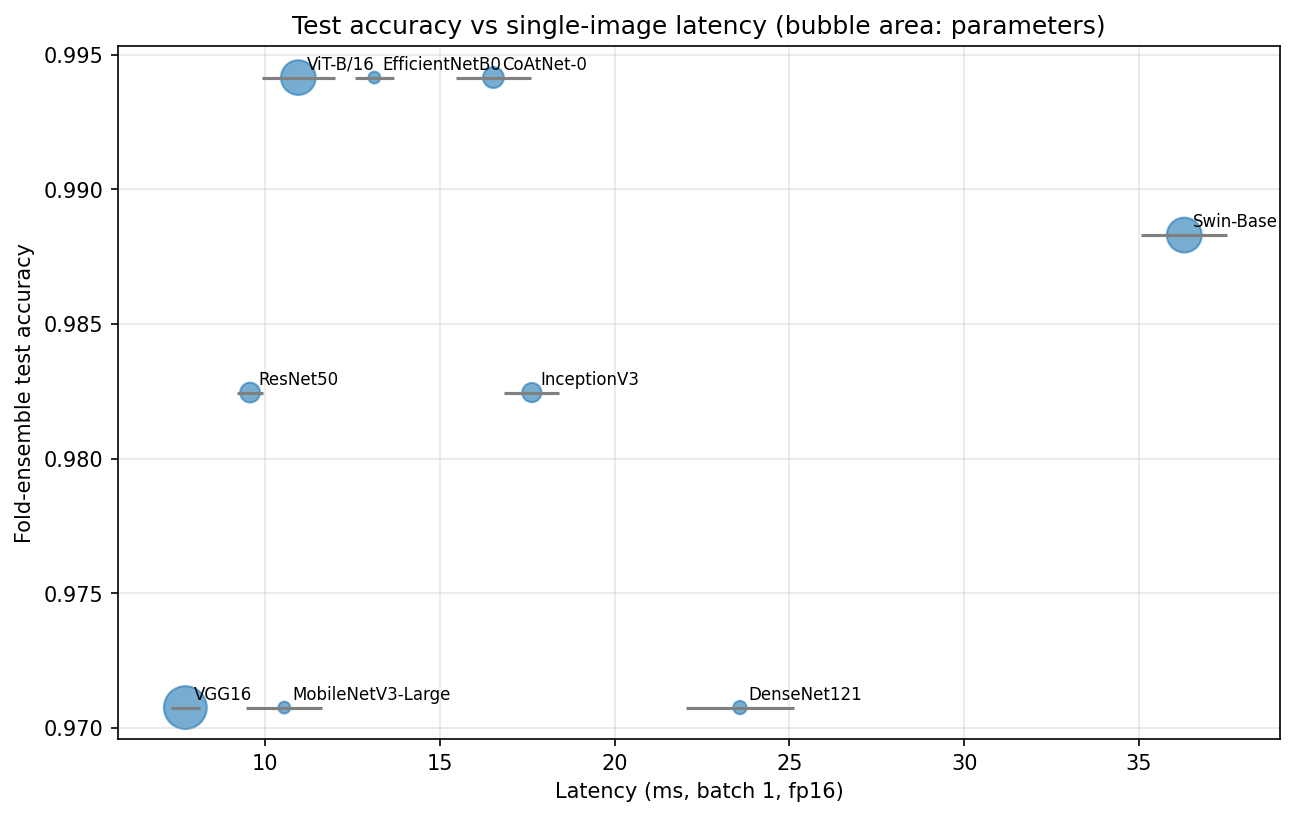
\includegraphics[width=\linewidth]{binary-detection/plots/18_accuracy_vs_latency.png}
\caption{Binary detection: fold-ensemble test accuracy against single-image latency for every model.}
\label{fig:latency}
\end{figure}

\subsection{Interpretability and Shortcut Analysis}
\label{sec:interpretability}

Table~\ref{tab:attention} summarises four measurements of whether the models rely on the head. The share of Grad-CAM energy outside the head is below the share of a uniform map for most models and classes, which on its own would suggest attention concentrated on the head. ViT-B/16 is the exception in detection, with 42.6\% of its Grad-CAM energy and 42.1\% of its attention rollout outside the head on tumour-negative images, against 35.6\% for a uniform map, and CoAtNet-0 places 41.7\% outside the head on the single glioma test image. Occlusion maps, which are computed the same way for every architecture, place between 0.7\% (VGG16) and 19.4\% (EfficientNetB0) of the sensitivity outside the head in detection and between 6.6\% and 12.4\% in classification. The EfficientNetB0 maps are shown in Figure~\ref{fig:gradcam}; the outside-head energy of every model is plotted in Supplementary Figure~S14, the occlusion maps in Supplementary Figures~S15 and S16, the masking test in Supplementary Figure~S17, the Grad-CAM maps of every model in Supplementary Figures~S18 to S26, and the per-class values and shortcut p-values in Supplementary Tables~S7 and S8. Test accuracy against the distance to the development pool is given in Supplementary Table~S5 and Figure~S12.

\begin{table*}[htbp]
\centering
\caption{Reliance on the head and on the background. Grad-CAM: share of map energy outside the head mask, the average of the per-class means over test images (uniform map: 0.34 binary, 0.25 multiclass, averaged the same way). Occlusion: share of occlusion sensitivity outside the head on 16 (binary) and 17 (multiclass) test images. Masking: mean fold accuracy on test images with the background set to zero (head only) or the head set to zero (background only). Shortcut: accuracy on background-only test images of a model trained on background-only images; majority-class rate 0.626 (binary) and 0.689 (multiclass); $^{*}$ above chance after Holm correction.}
\label{tab:attention}
\small
\setlength{\tabcolsep}{3pt}
\begin{tabular*}{\textwidth}{@{\extracolsep{\fill}}lcccccccccc@{}}
\toprule
 & \multicolumn{5}{c}{Binary detection} & \multicolumn{5}{c}{Subtype classification} \\
\cmidrule(lr){2-6}\cmidrule(l){7-11}
Model & Grad-CAM & Occl. & Head & Backgr. & Shortcut & Grad-CAM & Occl. & Head & Backgr. & Shortcut \\
\midrule
ResNet50 & 0.100 & 0.116 & 0.960 & 0.492 & 0.813$^{*}$ & 0.087 & 0.079 & 0.947 & 0.284 & 0.933$^{*}$ \\
VGG16 & 0.113 & 0.007 & 0.947 & 0.499 & 0.749$^{*}$ & 0.087 & 0.079 & 0.942 & 0.240 & 0.978$^{*}$ \\
DenseNet121 & 0.183 & 0.135 & 0.944 & 0.518 & 0.795$^{*}$ & 0.135 & 0.110 & 0.960 & 0.276 & 0.867$^{*}$ \\
EfficientNetB0 & 0.179 & 0.194 & 0.956 & 0.498 & 0.778$^{*}$ & 0.064 & 0.066 & 0.956 & 0.133 & 0.889$^{*}$ \\
MobileNetV3-Large & 0.112 & 0.111 & 0.937 & 0.533 & 0.678 & 0.077 & 0.071 & 0.951 & 0.338 & 0.933$^{*}$ \\
InceptionV3 & 0.147 & 0.167 & 0.945 & 0.657 & 0.795$^{*}$ & 0.122 & 0.099 & 0.947 & 0.218 & 0.978$^{*}$ \\
ViT-B/16 & 0.335 & 0.155 & 0.957 & 0.450 & 0.655 & 0.207 & 0.107 & 0.987 & 0.116 & 0.911$^{*}$ \\
Swin-Base & 0.172 & 0.182 & 0.968 & 0.517 & 0.830$^{*}$ & 0.102 & 0.122 & 0.996 & 0.169 & 0.911$^{*}$ \\
CoAtNet-0 & 0.164 & 0.089 & 0.964 & 0.444 & 0.795$^{*}$ & 0.231 & 0.124 & 0.982 & 0.156 & 0.822$^{*}$ \\
\bottomrule
\end{tabular*}
\end{table*}

The masking test agrees with the attention measurements. With the background set to zero, every model keeps most of its accuracy, between 93.7\% and 96.8\% in detection and between 94.2\% and 99.6\% in classification. With the head set to zero, detection accuracy falls to between 44.4\% and 53.3\% for every model except InceptionV3 (65.7\%), close to or below the majority-class rate of 62.6\%, and classification accuracy falls to between 11.6\% and 33.8\%, below its majority-class rate of 68.9\%. Models trained on full images therefore depend on the head.

The shortcut test shows that this is not the whole story. When each backbone is retrained on images whose head region is set to zero, it learns to predict the label from the background alone well above chance (Figure~\ref{fig:shortcut}). In detection, seven of the nine background-only models exceed the majority-class rate of 62.6\% after Holm correction, reaching 83.0\% for Swin-Base, 81.3\% for ResNet50 and 77.8\% for EfficientNetB0, with background-only AUCs up to 0.889; only MobileNetV3-Large (67.8\%) and ViT-B/16 (65.5\%) are not significant. In classification all nine are significant, with background-only accuracies between 82.2\% and 97.8\% against a majority-class rate of 68.9\%, and background-only AUCs between 0.972 and 1.000. The background, borders and framing of these public collections therefore carry substantial label information, in the multiclass pool almost enough to solve the test set without any brain. The models trained on full images do not need the background to perform well, as the masking test shows, but the data do not prevent them from using it, and the accuracies in Tables~\ref{tab:binary-results} and \ref{tab:multiclass-results} cannot be taken as proof that pathology has been learned.

\begin{figure*}[htbp]
\centering
\begin{subfigure}{\textwidth}
\centering
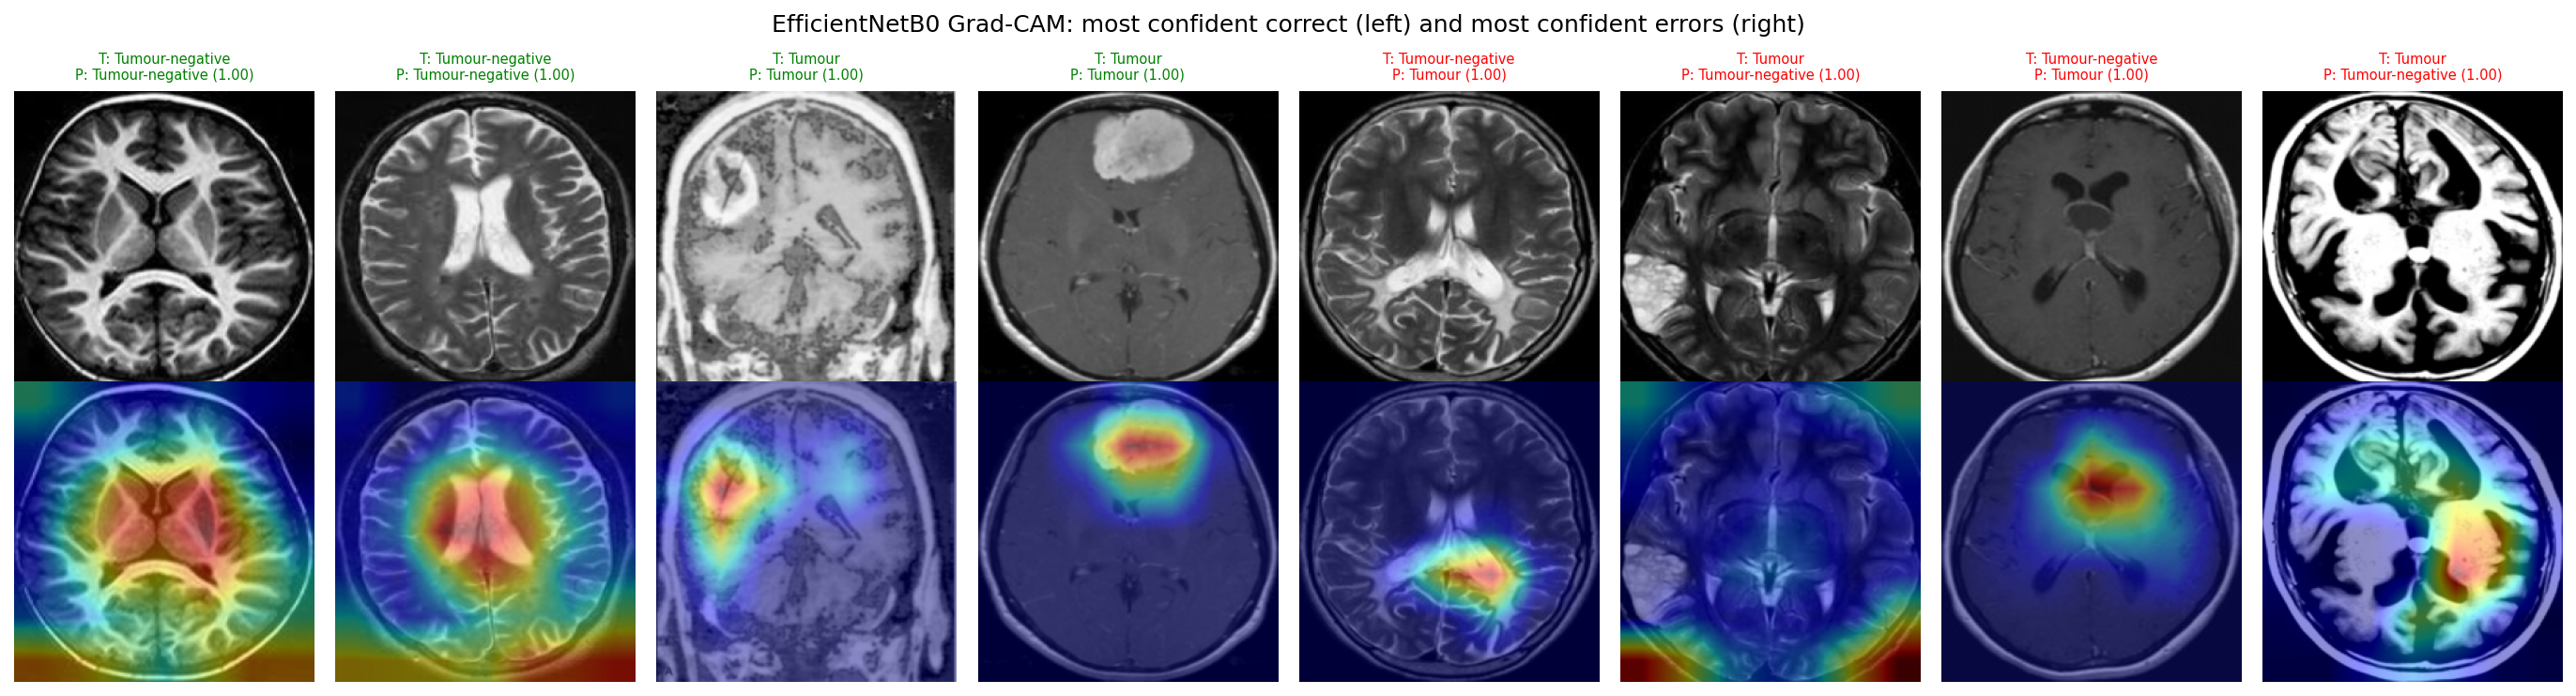
\includegraphics[width=\linewidth]{binary-detection/plots/13_gradcam_efficientnetb0.png}
\caption{Binary detection.}
\end{subfigure}
\\[4pt]
\begin{subfigure}{\textwidth}
\centering
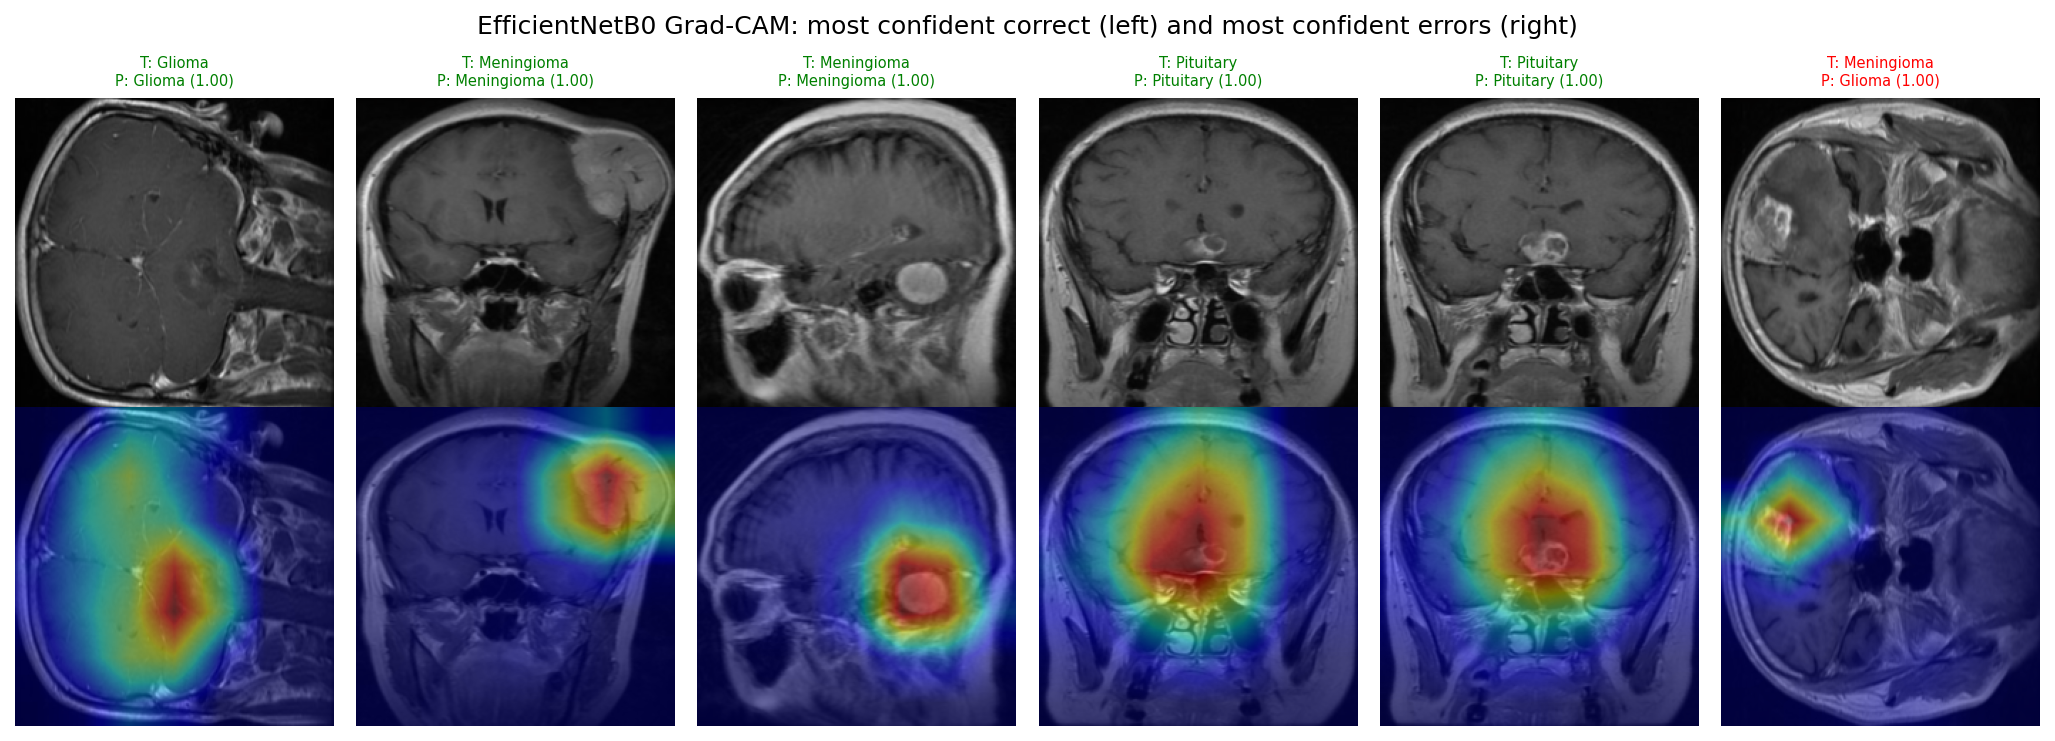
\includegraphics[width=\linewidth]{classification/plots/13_gradcam_efficientnetb0.png}
\caption{Subtype classification.}
\end{subfigure}
\caption{Grad-CAM maps of \textbf{EfficientNetB0}, the deployed architecture, on its most confident correct and most confident wrong test predictions, from the fold with the lowest validation loss.}
\label{fig:gradcam}
\end{figure*}

\begin{figure*}[htbp]
\centering
\begin{subfigure}{0.49\textwidth}
\centering
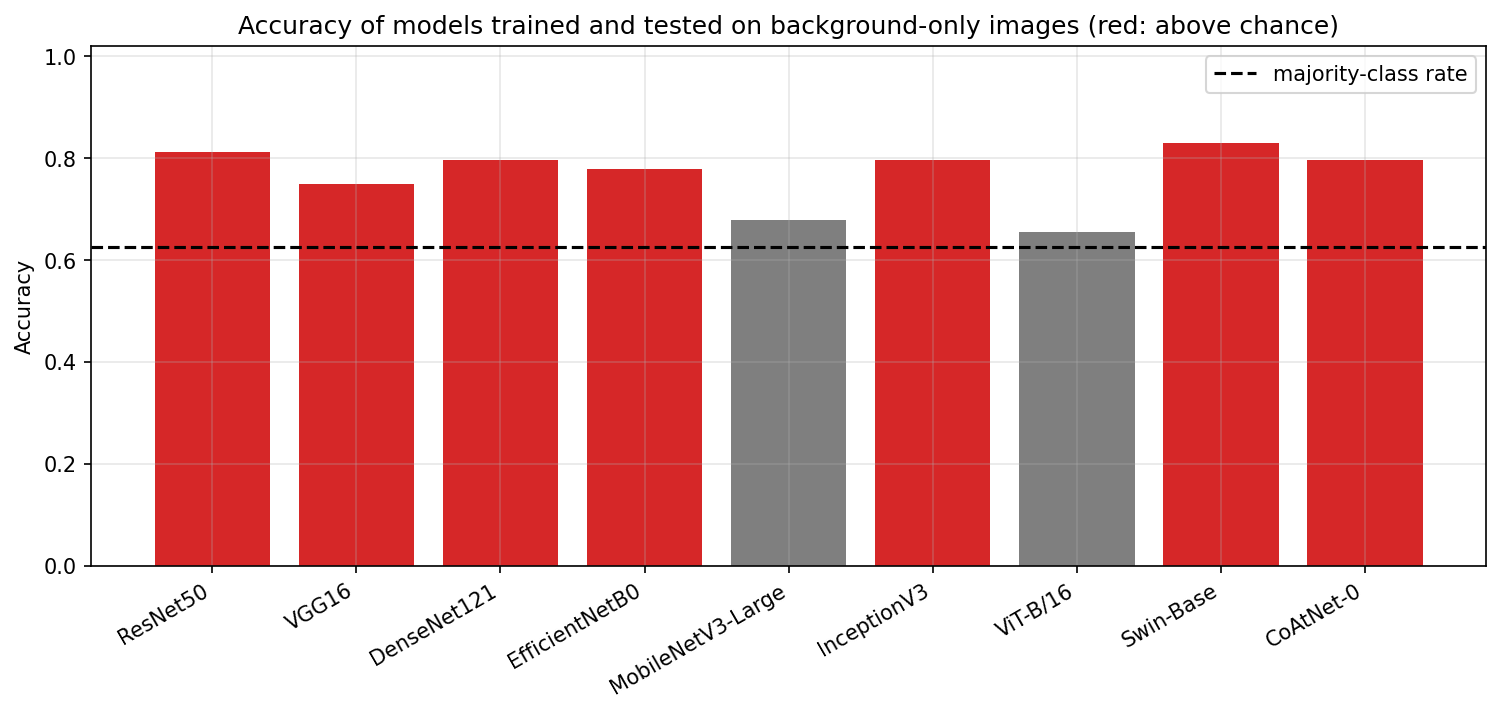
\includegraphics[width=\linewidth]{binary-detection/plots/17_shortcut_test.png}
\caption{Binary detection.}
\end{subfigure}
\hfill
\begin{subfigure}{0.49\textwidth}
\centering
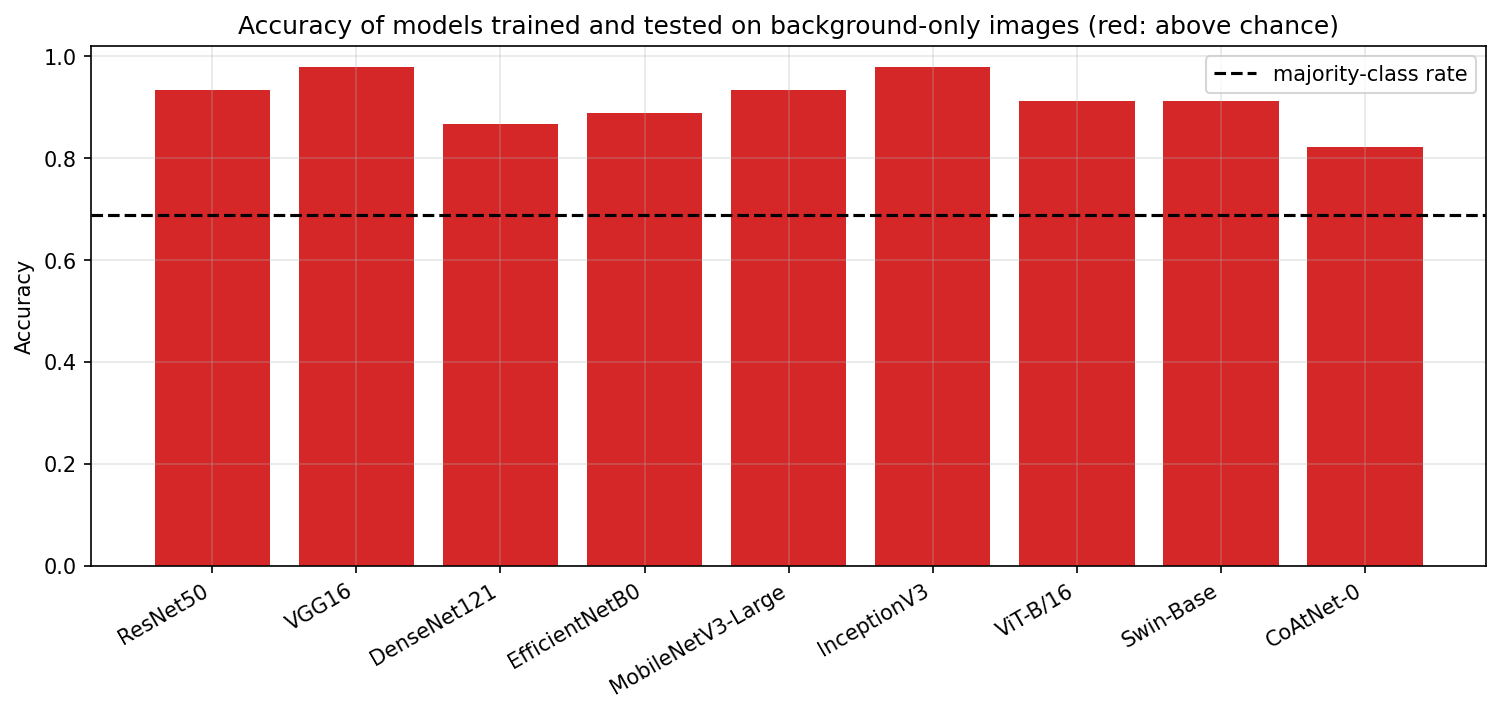
\includegraphics[width=\linewidth]{classification/plots/17_shortcut_test.png}
\caption{Subtype classification.}
\end{subfigure}
\caption{Shortcut test: accuracy on background-only test images of models trained on background-only images (fold 0); red bars are significantly above the majority-class rate after Holm correction.}
\label{fig:shortcut}
\end{figure*}

\subsection{Comparison with Existing Literature}
\label{sec:comparison}

Table~\ref{tab:literature-comparison} places the fold-ensemble results beside published figures for the same architectures. The comparison is for orientation only. The published studies mostly evaluate on the 3,064-image Cheng collection or on official partitions without deduplication, whereas the results here are measured after removing 63.57\% of the binary pool and 18.84\% of the multiclass pool as near-duplicates and after splitting by group; removing near-duplicates removes exactly the images most likely to have inflated a score. The multiclass result rests on 45 test images and is not comparable with results on full test splits. The models here also share one training configuration rather than being tuned individually.

\begin{table*}[htbp]
\centering
\caption{Present results beside previously published studies. ``This work'' is fold-ensemble accuracy on the held-out test set: 171 images for binary detection and 45 for subtype classification.}
\label{tab:literature-comparison}
\small
\begin{tabular*}{\textwidth}{@{\extracolsep{\fill}}llcccc@{}}
\toprule
Study & Model & Dataset size & Task & Reported accuracy & This work \\
\midrule
Talo et al. (2019) \cite{ref16} & ResNet50 & 253 & Binary & 95.23\% & 98.25\% \\
Khan et al. (2020) \cite{ref23} & VGG16 & 3,064 & Binary & 98.69\% & 97.08\% \\
Noreen et al. (2020) \cite{ref24} & DenseNet121 & 3,064 & Binary & 99.51\% & 97.08\% \\
Rehman et al. (2020) \cite{ref25} & InceptionV3 & 3,064 & Binary & 99.34\% & 98.25\% \\
Ghassemi et al. (2020) \cite{ref26} & EfficientNet & 3,064 & Binary & 98.87\% & 99.42\% \\
Deepak and Ameer (2019) \cite{ref15} & InceptionV3 & 3,064 & Multiclass & 97.50\% & 100.00\% \\
\bottomrule
\end{tabular*}
\end{table*}

Three conclusions about architecture can be drawn from these experiments, and one cannot. First, under an equal optimisation budget every backbone family reaches 97\% to 99\% detection accuracy, and the differences between families are not significant on 171 test images, so this benchmark gives no support to the claim that transformers, hybrids or convolutional networks are better suited to the task. Second, cost differs by two orders of magnitude for statistically indistinguishable accuracy, which makes cost the deciding factor in practice: EfficientNetB0 matches the leaders with 4.01 million parameters and 0.77 GFLOPs and has the second-highest throughput, which is why it is the architecture deployed in the accompanying application. Third, cross-validation spread is as large as the gaps between models, so single-run leaderboards on collections of this size cannot rank architectures. What cannot be concluded is that any of these models has learned tumour morphology rather than properties of the source collections, since background-only models reach 83\% detection and 98\% subtype accuracy.

\section{Conclusion}
\label{sec:conclusion}

This study benchmarked nine ImageNet-pretrained backbones for brain tumour detection and subtype classification with one pipeline: label-aware perceptual-hash deduplication and group-aware splitting before any training, an equal number of optimiser steps for every model, five-fold cross-validation with fold ensembles, bootstrap confidence intervals and Holm-corrected McNemar tests, calibration analysis, measured efficiency, and attention and shortcut audits for every model. Deduplication removed 63.57\% of the binary and 18.84\% of the multiclass images, and the leakage audit found no test image near a development image. On 171 binary test images, CoAtNet-0, EfficientNetB0 and ViT-B/16 reached 99.42\% accuracy, and no model differed significantly from any other; only VGG16 and MobileNetV3-Large were separable from the leader by the bootstrap interval of the accuracy gap. The multiclass split was dominated by one group of 1,431 images, so its test set of 45 images, on which six models were error-free and three made one error, cannot rank the models. Temperature scaling fitted on near-separable validation folds made calibration worse for most models. Most importantly, models retrained on background-only images exceeded chance for 7 of 9 detection and all 9 classification backbones, with up to 83.04\% and 97.78\% accuracy, so the public collections used here and in much of the literature carry label information outside the brain, and high accuracy on them does not establish that pathology has been learned. The principal limitations are that the images are public two-dimensional slices of unknown MRI sequence without patient identifiers, so grouping by image similarity is only a proxy for a patient-level split; that the binary negative class is tumour-negative rather than certified normal; that no external validation set was available; and that every model was trained once per fold with one seed and one shared configuration. Future work should split by patient where identifiers exist, use a smaller grouping tolerance or a different grouping criterion for the multiclass pool so that its test set represents every class, remove or standardise the image border before training and repeat the shortcut test, fit calibration on larger held-out sets, and validate externally on multi-sequence and three-dimensional institutional data before any clinical claim is made. The notebooks, splits, metrics and checkpoints are released so that both the results and their caveats can be reproduced.

\section*{Declaration of competing interest}

The authors declare that they have no known competing financial interests or personal relationships that could have appeared to influence the work reported in this paper.

\section*{Data availability}

All datasets used in this study are publicly available and are cited in Section~\ref{sec:data}. The notebooks, the split of every image, the per-run metrics and the trained checkpoints are available at the repository given in \ref{app:code}.

\section*{Supplementary material}

Supplementary material associated with this article is provided in a separate file. It contains the deduplication threshold sweep (Supplementary Table~S1), the temperature, threshold and test result of every run (Tables~S2 and S3), the per-class test metrics of every model (Table~S4), test accuracy by distance to the development pool (Table~S5), the complete efficiency measurements (Table~S6), the per-class outside-head energy (Table~S7), the shortcut test with its p-values (Table~S8), and Supplementary Figures~S1 to S26, covering dataset overviews, deduplication, cross-label pairs, groups and leakage, augmentation, training curves, receiver operating characteristic and precision--recall curves, McNemar p-values, confusion matrices, reliability diagrams, accuracy by distance, outside-head energy, occlusion maps, the masking test, accuracy against latency, and the Grad-CAM maps of every model.

\begin{thebibliography}{99}

\bibitem{ref1} E. I. Zacharaki, S. Wang, S. Chawla, et al., ``Classification of brain tumor type and grade using MRI texture and shape in a machine learning scheme,'' Magnetic Resonance in Medicine, vol. 62, no. 6, pp. 1609-1618, 2009.

\bibitem{ref2} S. Bauer, R. Wiest, L. P. Nolte, and M. Reyes, ``A survey of MRI-based medical image analysis for brain tumor studies,'' Physics in Medicine and Biology, vol. 58, no. 13, pp. R97-R129, 2013.

\bibitem{ref3} N. Gordillo, E. Montseny, and P. Sobrevilla, ``State of the art survey on MRI brain tumor segmentation,'' Magnetic Resonance Imaging, vol. 31, no. 8, pp. 1426-1438, 2013.

\bibitem{ref4} K. Simonyan and A. Zisserman, ``Very deep convolutional networks for large-scale image recognition,'' arXiv preprint arXiv:1409.1556, 2014.

\bibitem{ref5} J. Cheng, W. Huang, S. Cao, et al., ``Enhanced performance of brain tumor classification via tumor region augmentation and partition,'' PLoS ONE, vol. 10, no. 10, p. e0140381, 2015.

\bibitem{ref6} K. He, X. Zhang, S. Ren, and J. Sun, ``Deep residual learning for image recognition,'' in Proc. IEEE Conf. Comput. Vis. Pattern Recognit. (CVPR), 2016, pp. 770-778.

\bibitem{ref7} C. Szegedy, V. Vanhoucke, S. Ioffe, J. Shlens, and Z. Wojna, ``Rethinking the inception architecture for computer vision,'' in Proc. IEEE Conf. Comput. Vis. Pattern Recognit. (CVPR), 2016, pp. 2818-2826.

\bibitem{ref9} G. Huang, Z. Liu, L. Van Der Maaten, and K. Q. Weinberger, ``Densely connected convolutional networks,'' in Proc. IEEE Conf. Comput. Vis. Pattern Recognit. (CVPR), 2017, pp. 4700-4708.

\bibitem{ref12} J. Seetha and S. S. Raja, ``Brain tumor classification using convolutional neural networks,'' Biomedical and Pharmacology Journal, vol. 11, no. 3, p. 1457, 2018.

\bibitem{ref13} A. L. Beam and I. S. Kohane, ``Big data and machine learning in health care,'' JAMA, vol. 319, no. 13, pp. 1317-1318, 2018.

\bibitem{ref14} J. De Fauw, J. R. Ledsam, B. Romera-Paredes, et al., ``Clinically applicable deep learning for diagnosis and referral in retinal disease,'' Nature Medicine, vol. 24, no. 9, pp. 1342-1350, 2018.

\bibitem{ref15} S. Deepak and P. M. Ameer, ``Brain tumor classification using deep CNN features via transfer learning,'' Computers in Biology and Medicine, vol. 111, p. 103345, 2019.

\bibitem{ref16} M. Talo, U. B. Baloglu, \"O. Y{\i}ld{\i}r{\i}m, and U. R. Acharya, ``Application of deep transfer learning for automated brain abnormality classification using MR images,'' Cognitive Systems Research, vol. 54, pp. 176-188, 2019.

\bibitem{ref18} M. Tan and Q. Le, ``EfficientNet: Rethinking model scaling for convolutional neural networks,'' in Proc. Int. Conf. Mach. Learn. (ICML), 2019, pp. 6105-6114.

\bibitem{ref19} A. Howard, M. Sandler, G. Chu, et al., ``Searching for MobileNetV3,'' in Proc. IEEE/CVF Int. Conf. Comput. Vis. (ICCV), 2019, pp. 1314-1324.

\bibitem{ref23} M. A. Khan, I. Ashraf, M. Alhaisoni, et al., ``Multimodal brain tumor classification using deep learning and robust feature selection: A machine learning application for radiologists,'' Diagnostics, vol. 10, no. 8, p. 565, 2020.

\bibitem{ref24} N. Noreen, S. Palaniappan, A. Qayyum, I. Ahmad, M. Imran, and M. Shoaib, ``A deep learning model based on concatenation approach for the diagnosis of brain tumor,'' IEEE Access, vol. 8, pp. 55135-55144, 2020.

\bibitem{ref25} A. Rehman, S. Naz, M. I. Razzak, F. Akram, and M. Imran, ``A deep learning-based framework for automatic brain tumors classification using transfer learning,'' Circuits, Systems, and Signal Processing, vol. 39, no. 2, pp. 757-775, 2020.

\bibitem{ref26} N. Ghassemi, A. Shoeibi, and M. Rouhani, ``Deep neural network with generative adversarial networks pre-training for brain tumor classification based on MR images,'' Biomedical Signal Processing and Control, vol. 57, p. 101678, 2020.

\bibitem{ref28} A. Dosovitskiy, L. Beyer, A. Kolesnikov, et al., ``An image is worth 16x16 words: Transformers for image recognition at scale,'' in Proc. Int. Conf. Learn. Represent. (ICLR), 2021.

\bibitem{ref29} Z. Liu, Y. Lin, Y. Cao, et al., ``Swin transformer: Hierarchical vision transformer using shifted windows,'' in Proc. IEEE/CVF Int. Conf. Comput. Vis. (ICCV), 2021, pp. 10012-10022.

\bibitem{ref30} Z. Dai, H. Liu, Q. V. Le, and M. Tan, ``CoAtNet: Marrying convolution and attention for all data sizes,'' in Advances in Neural Information Processing Systems (NeurIPS), vol. 34, 2021, pp. 3965-3977.

\bibitem{ref32} S. Khan, M. Naseer, M. Hayat, S. W. Zamir, F. S. Khan, and M. Shah, ``Transformers in vision: A survey,'' ACM Computing Surveys, vol. 54, no. 10s, pp. 1-41, 2022.

\bibitem{guo2017} C. Guo, G. Pleiss, Y. Sun, and K. Q. Weinberger, ``On calibration of modern neural networks,'' in Proc. Int. Conf. Mach. Learn. (ICML), 2017, pp. 1321-1330.

\bibitem{selvaraju2017} R. R. Selvaraju, M. Cogswell, A. Das, R. Vedantam, D. Parikh, and D. Batra, ``Grad-CAM: Visual explanations from deep networks via gradient-based localization,'' in Proc. IEEE Int. Conf. Comput. Vis. (ICCV), 2017, pp. 618-626.

\bibitem{abnar2020} S. Abnar and W. Zuidema, ``Quantifying attention flow in transformers,'' in Proc. Annu. Meeting Assoc. Comput. Linguistics (ACL), 2020, pp. 4190-4197.

\bibitem{holm1979} S. Holm, ``A simple sequentially rejective multiple test procedure,'' Scandinavian Journal of Statistics, vol. 6, no. 2, pp. 65-70, 1979.

\bibitem{cbtrus} Q. T. Ostrom, M. Price, C. Neff, et al., ``CBTRUS statistical report: Primary brain and other central nervous system tumors diagnosed in the United States in 2016--2020,'' Neuro-Oncology, vol. 25, suppl. 4, pp. iv1-iv99, 2023, doi: \url{https://doi.org/10.1093/neuonc/noad149}

\bibitem{tummala2022} S. Tummala, S. Kadry, S. A. C. Bukhari, and H. T. Rauf, ``Classification of brain tumor from magnetic resonance imaging using vision transformers ensembling,'' Current Oncology, vol. 29, no. 10, pp. 7498-7511, 2022, doi: \url{https://doi.org/10.3390/curroncol29100590}

\bibitem{asiri2024} A. A. Asiri, A. Shaf, T. Ali, et al., ``Advancing brain tumor detection: Harnessing the Swin Transformer's power for accurate classification and performance analysis,'' PeerJ Computer Science, vol. 10, p. e1867, 2024, doi: \url{https://doi.org/10.7717/peerj-cs.1867}

\bibitem{shamshad2023} F. Shamshad, S. Khan, S. W. Zamir, et al., ``Transformers in medical imaging: A survey,'' Medical Image Analysis, vol. 88, p. 102802, 2023, doi: \url{https://doi.org/10.1016/j.media.2023.102802}

\bibitem{kapoor2023} S. Kapoor and A. Narayanan, ``Leakage and the reproducibility crisis in machine-learning-based science,'' Patterns, p. 100804, 2023, doi: \url{https://doi.org/10.1016/j.patter.2023.100804}

\bibitem{vangala2026} B. P. Vangala, S. Guda, L. Peddi, and N. Vangala, ``Scores that hold, benchmarks that leak: Measuring dataset contamination in public brain-tumor MRI classification,'' arXiv preprint arXiv:2610.00421, 2026.

\bibitem{ds1} N. Chakrabarty, ``Brain MRI images for brain tumor detection,'' Kaggle dataset, version 1, 2019. [Online]. Available: \url{https://www.kaggle.com/datasets/navoneel/brain-mri-images-for-brain-tumor-detection}

\bibitem{ds2} A. Hamada, ``Br35H :: Brain tumor detection 2020,'' IEEE DataPort, 2025, doi: \url{https://doi.org/10.21227/tbkk-q937}. Also available on Kaggle: \url{https://www.kaggle.com/datasets/ahmedhamada0/brain-tumor-detection}

\bibitem{ds3} S. Bhuvaji, A. Kadam, P. Bhumkar, S. Dedge, and S. Kanchan, ``Brain tumor classification (MRI),'' Kaggle dataset, 2020, doi: \url{https://doi.org/10.34740/KAGGLE/DSV/1183165}

\bibitem{ds4} J. Cheng, ``Brain tumor dataset,'' figshare, version 5, 2017, doi: \url{https://doi.org/10.6084/m9.figshare.1512427.v5}

\bibitem{ds5} MoundirB, ``Jun Cheng brain tumor MRI dataset JPG,'' Kaggle dataset, version 1, 2025. JPEG conversion of \cite{ds4}. [Online]. Available: \url{https://www.kaggle.com/datasets/moundir8/jun-cheng-brain-tumor-mri-dataset-jpg}

\end{thebibliography}

\FloatBarrier
\appendix

\section{Code Repository}
\label{app:code}

The notebooks for both tasks, which perform deduplication, splitting, training, evaluation and figure generation, are available together with their outputs (split tables, per-run metrics, plots and the exported checkpoints) at \url{https://github.com/parthmital/NeuroScan-AI}, in the folder \texttt{Materials/Notebooks}.

\end{document}
